\documentclass[USenglish, a4paper, thm-restate,numberwithinsect, cleveref]{lipics-v2021}

\pdfoutput=1 %uncomment to ensure pdflatex processing (mandatatory e.g. to submit to arXiv)
\hideLIPIcs  %uncomment to remove references to LIPIcs series (logo, DOI, ...), e.g. when preparing a pre-final version to be uploaded to arXiv or another public repository


\usepackage{graphicx}

\usepackage{amsmath,amsthm,amssymb,amsfonts}
\usepackage{nicefrac}
\usepackage{hyperref}
\usepackage{cleveref}
\crefname{appendix}{Appendix}{Appendices}
\Crefname{appendix}{Appendix}{Appendices}
\usepackage{xspace}

\usepackage{tabularx}
\usepackage{cite}
\usepackage{mathtools}
\usepackage{tikz}
\usetikzlibrary{arrows.meta,calc,positioning,fit,decorations.pathreplacing,decorations.pathmorphing,backgrounds,shapes.geometric}
\tikzset{
  vertex/.style={circle,draw=black!75,fill=white,inner sep=0pt,minimum size=5.2mm},
  smallv/.style={circle,draw=black!75,fill=white,inner sep=0pt,minimum size=3.2mm},
  root/.style={vertex,fill=black!18,draw=black,line width=.9pt},
  cycleedge/.style={black,line width=1pt},
  blueforest/.style={witnessblue,line width=1pt},
  orangeforest/.style={witnessorange,line width=1pt,dash pattern=on 3pt off 2pt},
  removed/.style={black!35,line width=.8pt},
  panel/.style={font=\small},
}

\definecolor{witnessblue}{HTML}{0072B2}
\definecolor{witnessorange}{HTML}{D55E00}
\definecolor{auxgreen}{HTML}{009E73}
\definecolor{auxpurple}{HTML}{7A3E9D}
\definecolor{complexitygreen}{HTML}{CFEAD6}
\definecolor{complexityred}{HTML}{F4CCCC}
\definecolor{complexitygray}{HTML}{DDDDDD}

\tikzstyle{knoten}=[circle,fill=white,draw=black,minimum size=7pt,inner sep=2pt]

\newcommand{\Oh}{\mathcal{O}}

\newcommand{\problemdef}[3]{
	\begin{center}\fbox{
	\begin{minipage}{0.95\textwidth}
        \vspace{3pt}
		\noindent
		\textsc{#1}
		\vspace{5pt}\\
		\setlength{\tabcolsep}{3pt}
		\begin{tabularx}{\textwidth}{@{}lX@{}}
			\text{Input:}     & #2 \\
			\text{Question:}  & #3
		\end{tabularx}
	\end{minipage}}
	\end{center}
}

\newcommand{\Gossip}{\textnormal{\textsc{Gossiping}}\xspace}


\usepackage[textsize=footnotesize,color=green!40]{todonotes}

\newcommand{\ralf}[1]{{\color{purple}[R: #1]}}
\newcommand{\ralfcomment}[2][]{\todo[color=purple!30,#1]{R: #2}}
\newcommand{\ralfcommenti}[1]{\ralfcomment[inline]{#1}}

\newcommand{\george}[1]{{\color{blue}[G: #1]}}
\newcommand{\georgecomment}[2][]{\todo[color=blue!30,#1]{G: #2}}
\newcommand{\georgecommenti}[1]{\georgecomment[inline]{#1}}

\newcommand{\paul}[1]{{\color{green}[P: #1]}}
\newcommand{\paulcomment}[2][]{\todo[color=green!30,#1]{P: #2}}
\newcommand{\paulcommenti}[1]{\paulcomment[inline]{#1}}

\title{Gossiping and the Characterization by T-Graphs and M-Graphs}

\titlerunning{Gossiping and the Characterization by T-Graphs and M-Graphs}

\ccsdesc[500]{Mathematics of computing~Graph algorithms}
\keywords{Gossiping, temporal connectivity, label-connected graphs, spanning trees}

\author{Ralf Klasing}{CNRS, LaBRI, Université de Bordeaux, Talence, France}{ralf.klasing@labri.fr}{https://orcid.org/0009-0004-9421-8525}{Partially supported by the French ANR, project ANR-22-CE48-0001 (TEMPOGRAL)}

\author{George B. Mertzios}{Department of Computer Science, Durham University, UK}{george.mertzios@durham.ac.uk}{https://orcid.org/0000-0001-7182-585X}{Supported by the EPSRC grant EP/P020372/1.}

\author{Hendrik Molter}{Chair for Algorithm Engineering, Hasso Plattner Institute, Potsdam, Germany \and Department of Computer Science, Ben-Gurion~University~of~the~Negev, 
	Beer-Sheva, 
	Israel}{hendrik.molter@hpi.de}{https://orcid.org/0000-0002-4590-798X}{Supported by the Israel Science Foundation, grant nr.~1470/24, by the European Union's Horizon Europe research and innovation programme under grant agreement 949707, by the European Research Council, grant nr.~101039913 (PARAPATH), and by the Deutsche Forschungsgemeinschaft (DFG, German Research Foundation) -- 565381415.}
	
\author{Nils Morawietz}{Institute of Computer Science, Friedrich Schiller University Jena,  Germany}{nils.morawietz@uni-jena.de}{https://orcid.org/0000-0002-7283-4982}{%Partially supported by the French ANR, project ANR-22-CE48-0001 (TEMPOGRAL)
}

\author{Paul G. Spirakis}{School  of Computer Science and Informatics, University of Liverpool, UK}{p.spirakis@liverpool.ac.uk}{https://orcid.org/0000-0001-5396-3749}{Supported by the EPSRC grant EP/P02002X/1.}

\acknowledgements{The authors declare the use of Generative AI as follows:
During the preparation of this manuscript, we used the large language
models ChatGPT (OpenAI) and Claude (Anthropic) for mathematical
brainstorming, literature discovery, proof writing, consistency checks, and language
editing. The authors subsequently checked and revised all mathematical
arguments, bibliographic claims, and formulations and take full
responsibility for the manuscript.}

\authorrunning{R. Klasing, G. B. Mertzios, H. Molter, N. Morawietz, and P. G. Spirakis}

\Copyright{Ralf Klasing, George B. Mertzios, Hendrik Molter, Nils Morawietz, and Paul G. Spirakis}

\nolinenumbers %uncomment to disable line numbering

\begin{document}
\renewcommand{\theHtheorem}{\thesection.\arabic{theorem}}
\providecommand{\theHlemma}{}
\renewcommand{\theHlemma}{\thesection.\arabic{theorem}}
\providecommand{\theHcorollary}{}
\renewcommand{\theHcorollary}{\thesection.\arabic{theorem}}
\maketitle
\begin{abstract}
In the classical gossiping setting, each participant initially knows a
distinct piece of information. Whenever two participants call each
other, they exchange everything they currently know. An undirected
multigraph is label-connected if its edges can be ordered as calls so
that every participant learns all information, using each edge at most
once. Equivalently, it admits a temporal labeling that makes it
connected by strict temporal paths. We give a self-contained proof of
the classical characterization: a multigraph is label-connected if and
only if it has at most one vertex, has two spanning trees sharing at
most one edge, or admits a cycle of length at least four and two
spanning forests, all pairwise edge-disjoint, each forest having four
components that meet the cycle. The proof constructs a complete call
order from either witness and, conversely, obtains a witness by
contracting two-tree blocks and lifting a suitable quotient structure.
\end{abstract}

\section{Introduction}

Distributing information among participants is a basic task in
communication networks. In a peer-to-peer exchange, two participants
can share both their own information and everything they have learned
from earlier exchanges. When the available pairwise exchanges are
fixed, their order determines how far information can spread. We ask
whether these exchanges can be scheduled so that every participant
receives all information, without introducing additional exchanges.

The classical gossiping problem captures this question in a particularly
clean form.  Each participant initially knows a distinct piece of
information, and whenever two participants call each other, they
exchange everything they currently know.  If every pair may communicate,
$2n-4$ calls are necessary and sufficient for $n\geq4$
participants~\cite{BakerS72,HajnalMS72}.  We instead prescribe the
available calls by an undirected multigraph: vertices represent
participants, and each edge represents one call between its endpoints.
The task is to decide whether these calls can be ordered so that all
information reaches every participant.  Thus the difficulty lies not in
selecting sufficiently many calls, but in coordinating a fixed and
possibly highly constrained set of calls.

This question is also a temporal graph realization problem.
A temporal graph $(G,\lambda)$ consists of an undirected multigraph
$G=(V,E)$ and a labeling $\lambda\colon E\to\mathbb{N}$ assigning a time
to each edge. A \emph{strict temporal path} is a path whose edge labels
strictly increase in traversal order.
The temporal graph is \emph{temporally connected} if such
a path exists for every ordered pair of vertices. 
Each edge receives exactly one label.\footnote{We use the temporal-graph terminology of edge labels and the gossiping terminology of calls interchangeably: an edge represents a call, and its label specifies when that call takes place.}
Different edges may receive equal labels. However, we can give all edges
distinct labels while preserving the order of edges whose labels were
already different. Every strict temporal path is preserved, so it suffices
to consider a total order of the calls (\Cref{sec:preliminaries}).
Loops are irrelevant, and parallel edges
represent distinct calls. A graph with at most one vertex is a
yes-instance. Disconnected graphs are immediate no-instances.
% lax begin Lax630294.Gossiping
\problemdef{\Gossip}{An undirected multigraph $G=(V,E)$.}{Is there a
labeling $\lambda\colon E\to\mathbb{N}$ such that $(G,\lambda)$ is
temporally connected?}
Following the classical literature, we call a multigraph
\emph{label-connected} if it is a yes-instance of \Gossip.
% lax end
G\"obel, Cerdeira, and Veldman~\cite{gobel1991label} proved that
recognizing label-connected graphs is NP-complete. A classical characterization
describes the yes-instances using either two spanning trees (a
\emph{$T$-witness}) or a cycle together with two spanning forests (an
\emph{$M$-witness})~\cite{BuroschLM88,BuroschL92,Krumme96}.
We give a self-contained proof of this characterization using the
notation and multigraph conventions fixed in \Cref{sec:preliminaries}.

First, we construct a complete call order from either type of witness
(\Cref{app:construct-labeling}). For the converse, we contract maximal
vertex sets supporting two edge-disjoint spanning trees and analyze
the resulting quotient (\Cref{sec:necessity-self-contained}). The main
difficulty is choosing a quotient cycle so that its witness can be
lifted to the original graph while keeping the cycle and forests
edge-disjoint.

The contraction, exchange, and lifting framework follows Burosch and
Laborde~\cite{BuroschL92}; the closed-tree counting argument follows
Bumby~\cite{Bumby81} and Kleitman and Shearer~\cite{KleitmanS80}.
We give these arguments in full and use information paths in the
original graph to ensure that the lifted cycle and forests are
edge-disjoint.

\section{Preliminaries and the Characterization}
\label{sec:preliminaries}
We fix our graph and temporal-labeling conventions, define the two
spanning witnesses, and state the classical characterization. We also
recall the basic matroid notions used in the sufficiency proof.

\subparagraph*{Graphs.}
We use standard graph-theoretic terminology; see, for example,
Diestel~\cite{Die16}. Unless stated otherwise, graphs are finite
undirected multigraphs, with parallel edges treated as distinct. We
write $n=|V(G)|$ and $m=|E(G)|$. Degrees count multiplicities; the
maximum degree of the support is explicitly identified and denoted
by $\Delta$. For $X\subseteq V(G)$, let $G[X]$ be the induced subgraph
and $E[X]$ its edge set. For $F\subseteq E(G)$, the graph $(V(G),F)$
retains isolated vertices, and $V(F)$ is the set of endpoints of $F$.
We write $[a]=\{1,\ldots,a\}$ for a positive integer $a$, use $G-S$
and $G-F$ for vertex and edge deletion, and $A\setminus B$ for set difference.

% lax begin Lax630294.SpanningStructures
The \emph{support} of a multigraph is the simple graph obtained by
deleting loops and replacing each nonempty parallel class by one
edge. A path has no repeated vertices; a path consisting of one vertex
is allowed. A \emph{cycle} of length $\ell\geq1$ is a closed walk
$v_0e_1v_1\cdots e_\ell v_\ell$ with $v_\ell=v_0$, pairwise distinct
edges $e_1,\ldots,e_\ell$, and pairwise distinct vertices
$v_0,\ldots,v_{\ell-1}$; we identify it with the subgraph formed by
these vertices and edges. Thus a cycle of length one is a loop, and a
cycle of length two consists of two parallel edges. The length of a
path is its number of edges.
A forest contains no cycle; in particular, it contains no loop and no
pair of parallel edges.
A spanning forest includes every vertex, and isolated vertices count
as components. A spanning forest on $n$ vertices with $c$ components
has $n-c$ edges. A \emph{matching} is a set of pairwise vertex-disjoint edges.
Edge-disjoint subgraphs may share vertices.
% lax end

We discard loops in instances of \Gossip, since they do not
affect communication. Contraction of a connected vertex set identifies
its vertices, retains external parallel edges, and deletes the resulting
loops. We call the graph obtained by contracting one or more pairwise
disjoint connected vertex sets a \emph{quotient} of the original graph.
In the graphic matroid constructions, we also identify vertex sets that
need not be connected. There we explicitly retain all edges, including
resulting loops, to preserve the matroid ground set.

\subparagraph*{Temporal Connectivity.}
A general introduction to temporal graphs is given by Casteigts et
al.~\cite{casteigts2012time}; for the distinctions between simple,
strict, and proper temporal graphs, we follow Casteigts, Corsini, and
Sarkar~\cite{CasteigtsCS22}.
% lax begin Lax630294.Gossiping
A \emph{temporal labeling} of a multigraph $G=(V,E)$ is a function
$\lambda\colon E\to\mathbb{N}$ assigning one positive integer to each
edge. A \emph{strict temporal path} traverses edges
$e_1,\ldots,e_\ell$ with
$\lambda(e_1)<\cdots<\lambda(e_\ell)$. The temporal graph
$(G,\lambda)$ is \emph{temporally connected} if a strict temporal path
exists from $u$ to $v$ for every ordered pair $u,v\in V$.
Paths of length zero are allowed, so a graph with at most one vertex
is temporally connected. 
% lax end
Order the edges by their labels, placing edges with equal labels in
an arbitrary order, and assign distinct labels $1,\ldots,m$ in that
order. This preserves every strict comparison between original labels
and hence every strict temporal path. Thus every temporally connectable
graph admits a bijective labeling $\lambda\colon E\to[m]$.


A bijective temporal labeling defines a \emph{gossip scheme}, that is,
a total order of the calls. Initially each vertex knows its own distinct
secret; when an edge is called, its endpoints
exchange all secrets they currently know. After any prefix of the
order, a vertex $v$ knows the secret of a vertex $u$ if and only if
some strict temporal path from $u$ to $v$ uses only calls of that prefix. 
A gossip scheme is \emph{complete} if every vertex knows every
secret after all calls. Thus $(G,\lambda)$ is temporally connected if
and only if the corresponding gossip scheme is complete.

\subparagraph*{Spanning Witnesses.}
The classical characterization uses the following two types of
subgraphs. We follow the terminology of Burosch and Laborde and of
Krumme~\cite{BuroschL92,Krumme96}.
% lax begin Lax630294.TGraph
\begin{definition}[$T$-graph and $T$-witness]
A multigraph is a \emph{$T$-graph} if it has two spanning trees sharing
at most one edge.
We call such a pair a \emph{$T$-witness}.
\end{definition}
% lax end

The second witness type replaces the two almost edge-disjoint trees by
two forests connected through a common cycle.
% lax begin Lax630294.MGraph
\begin{definition}[$M$-witness and $M$-graph]\label{def:m-graph}
An \emph{$M$-witness} of a multigraph $G$ consists of pairwise
edge-disjoint subgraphs $C,F_1,F_2$, where $C$ is a cycle of length at
least four and each $F_i$ is a spanning forest with exactly four
components, each containing a vertex of $C$. A graph is an \emph{$M$-graph} if it
admits an $M$-witness and is not a $T$-graph. An $M$-witness is
\emph{minimum} if $|E(C)|$ is minimum among all $M$-witnesses of $G$.
\end{definition}
% lax end

In this terminology, $T$-graphs and $M$-graphs form disjoint classes.
The gossiping literature calls an $M$-witness a \emph{realizing set}. We use ``witness'' to emphasize its
algorithmic role. For statements that also
apply to $T$-graphs containing such a cycle-and-forests structure, we
say explicitly that the graph \emph{admits an $M$-witness}.

In intuitive descriptions and figures, we call $F_1$ the
\emph{\textcolor{witnessblue}{blue forest}} and $F_2$ the
\emph{\textcolor{witnessorange}{orange forest}}. In figures showing
witnesses, we consistently use blue for $F_1$ and orange for $F_2$,
and the same colors for the corresponding witness trees. We retain
the notation $F_1,F_2$ in formal statements.

\begin{figure}[t]
\centering
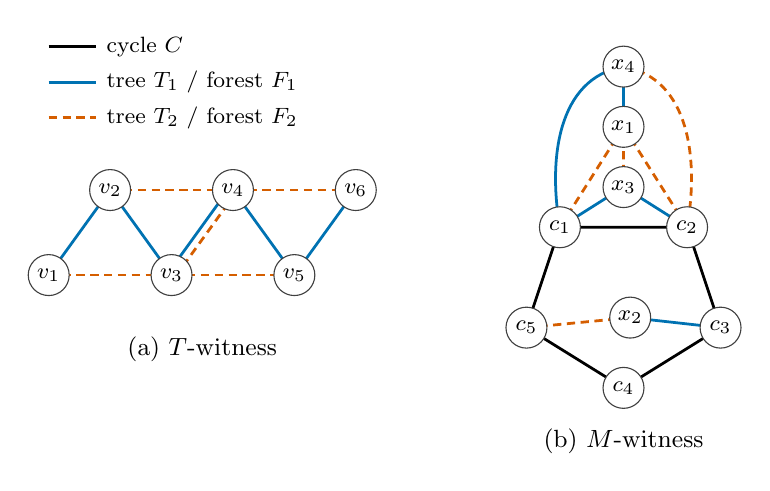
\begin{tikzpicture}[every node/.style={font=\footnotesize}]
% ---------------- panel (a): T-witness ----------------
\begin{scope}[x=0.78cm,y=0.9cm]
  \foreach \i/\x/\y in {1/0/0,2/1/1.2,3/2/0,4/3/1.2,5/4/0,6/5/1.2}
    \coordinate (v\i) at (\x,\y);
  % T_1: zigzag path, T_2: two straight lines plus the shared edge
  \draw[blueforest] (v1)--(v2)--(v3) (v4)--(v5)--(v6);
  \draw[orangeforest] (v1)--(v3)--(v5) (v2)--(v4)--(v6);
  % shared edge v3v4 drawn in both styles
  \draw[witnessblue,line width=1pt,transform canvas={xshift=-1.2pt,yshift=0.8pt}] (v3)--(v4);
  \draw[orangeforest,transform canvas={xshift=1.2pt,yshift=-0.8pt}] (v3)--(v4);
  \foreach \i in {1,...,6} \node[vertex] at (v\i) {$v_\i$};
  \node[panel] at (2.5,-1.05) {(a) $T$-witness};
\end{scope}
% ---------------- panel (b): M-witness ----------------
\begin{scope}[xshift=7.3cm,yshift=-0.2cm,scale=0.85,every node/.append style={transform shape=false}]
  \coordinate (c1) at (-0.95,0.95);
  \coordinate (c2) at (0.95,0.95);
  \coordinate (c3) at (1.45,-0.55);
  \coordinate (c4) at (0,-1.45);
  \coordinate (c5) at (-1.45,-0.55);
  \coordinate (x3) at (0,1.55);
  \coordinate (x1) at (0,2.45);
  \coordinate (x4) at (0,3.35);
  \coordinate (x2) at (0.1,-0.4);
  \draw[cycleedge] (c1)--(c2)--(c3)--(c4)--(c5)--(c1);
  \draw[blueforest] (x3)--(c1) (x3)--(c2) (x4) to[out=190,in=100] (c1) (x4)--(x1) (x2)--(c3);
  \draw[orangeforest] (x3)--(x1) (x1)--(c1) (x1)--(c2) (x4) to[out=-10,in=80] (c2) (x2)--(c5);
  \foreach \v/\l in {c1/c_1,c2/c_2,c3/c_3,c4/c_4,c5/c_5,x1/x_1,x2/x_2,x3/x_3,x4/x_4}
    \node[vertex] at (\v) {$\l$};
  \node[panel] at (0,-2.25) {(b) $M$-witness};
\end{scope}
% ---------------- legend ----------------
\begin{scope}[xshift=0cm,yshift=2.9cm]
  \draw[cycleedge] (0,0)--(0.6,0) node[right,text=black] {cycle $C$};
  \draw[blueforest] (0,-0.45)--(0.6,-0.45) node[right,text=black] {tree $T_1$ / forest $F_1$};
  \draw[orangeforest] (0,-0.9)--(0.6,-0.9) node[right,text=black] {tree $T_2$ / forest $F_2$};
\end{scope}
\end{tikzpicture}
\caption{The two witness types.
(a) A $T$-witness: two spanning trees $T_1$ (solid) and $T_2$ (dashed)
that share only the edge $v_3v_4$. (b) An $M$-witness on nine vertices:
the black edges form the cycle $C$, and the blue and orange edges form
spanning forests with four components each, all meeting $C$. The graph
in (b) has $15=2n-3$ edges, but it is not a $T$-graph (see the text). We use it as a running example
in \Cref{fig:labeling-example}.}
\label{fig:m-graph}
\end{figure}

\Cref{fig:m-graph} shows both witness types. The graph in
\Cref{fig:m-graph}(b) has nine vertices and $15=2n-3$ edges, which is
exactly the number of edges of two spanning trees sharing one edge.
Nevertheless, it is not a $T$-graph: the five vertices
$c_1,c_2,x_1,x_3,x_4$ induce nine edges, but at most
$2(5-1)=8$ of them lie in a union of two forests. Hence, every union of
two forests has at most $2n-4$ edges. We use this graph as a running
example.

\subparagraph*{Matroids.}
We use standard matroid terminology; see Oxley~\cite{Oxley2011}.
A \emph{matroid} $M=(E,\mathcal{I})$ has a finite ground set $E$ and
a family $\mathcal{I}\subseteq2^E$ of \emph{independent sets} containing
$\varnothing$, closed under subsets, and satisfying the exchange
axiom: for $A,B\in\mathcal{I}$ with $|A|<|B|$, some $b\in B\setminus A$
has $A\cup\{b\}\in\mathcal{I}$. We also write $\mathcal{I}(M)$ for
this family. A \emph{basis} is an inclusion-maximal independent set;
all bases have the same size, the \emph{rank} $r(M)$. A \emph{loop}
belongs to no independent set.

The \emph{graphic matroid} $M(G)$ of a multigraph $G=(V,E)$ has ground
set $E$ and independent sets $F$ for which $(V,F)$ is a forest.
Its loops are exactly those of $G$, and parallel edges remain distinct
elements. 
An independence oracle decides whether a given subset of the ground
set is independent. We use such oracles only for graphic matroids of
quotients on four vertices.

\subparagraph*{The Characterization.}
The following theorem characterizes the label-connected multigraphs
by the two witness types. We prove sufficiency in
\Cref{app:construct-labeling} and necessity in
\Cref{sec:necessity-self-contained}.
\label{sec:witnesses}

% lax begin Lax630294.Characterization
\begin{theorem}[{\cite{BuroschLM88,BuroschL92,Krumme96}}]\label{thm:characterization}
Let $G$ be a multigraph. Then $G$ is a yes-instance of \Gossip if and only
if at least one of the following conditions holds:
\begin{enumerate}
\item\label{Gtrivial} $G$ has at most one vertex;
\item\label{GisT} $G$ is a $T$-graph;
\item\label{GisM} $G$ is an $M$-graph.
\end{enumerate}
\end{theorem}
% lax end


% lax begin Lax630294Proofs.isLabelConnected_iff
\section{Sufficiency: Constructing a Temporal Labeling}
\label{app:construct-labeling}

We first describe how the components of the two forests meet the
cycle of an $M$-witness in an $M$-graph. An \emph{interval} of the
cycle is a nonempty set of consecutive cycle vertices, forming a
path; a single vertex is allowed. The following lemma states that
the four components of each forest meet the cycle in the same four
intervals. The four edges between consecutive intervals can be paired
by taking every other edge in cyclic order. Each pair is a matching
whose endpoints provide one root in each component of either forest.
We prove this below.

\begin{lemma}[{\cite[Corollary~1 and proof of Theorem~3]{Krumme96}}]\label{lem:four-intervals}
Let $G$ be an $M$-graph, and let $(C,F_1,F_2)$ be an $M$-witness of $G$.
There is a partition of $V(C)$ into four nonempty consecutive intervals
$X_1,X_2,X_3,X_4$, indexed in cyclic order, with the following properties:
\label{lem:structured-m-witness}%
\begin{itemize}
\item \emph{Common intervals.} For each forest $F_j$, the intersections
of its four components with $V(C)$ are exactly $X_1,X_2,X_3,X_4$.
\item \emph{Alternating matchings.} Let $b_i$ be the cycle edge joining
$X_i$ to $X_{i+1}$, with indices modulo four. Then
$B_1=\{b_1,b_3\}$ and $B_2=\{b_2,b_4\}$ are edge-disjoint matchings.
Every component of each forest contains exactly one vertex of $V(B_1)$
and exactly one vertex of $V(B_2)$.
\end{itemize}
\end{lemma}

Krumme calls $b_1,\ldots,b_4$ the \emph{essential} edges.
If an interval consists of a single vertex, then $B_1$ and $B_2$
share that vertex. Thus the two matchings need not have disjoint
vertex sets.
In particular, both forests of an $M$-witness of an $M$-graph can be
rooted\footnote{Rooting a forest means choosing one vertex as the root of each tree component.} at the same four vertices, namely at the endpoints of~$B_1$.
The
labeling construction of \Cref{lem:construct-labeling} instead roots
$F_1$ at the endpoints of $B_1$ and $F_2$ at those of $B_2$.

The classical constructions of Burosch and Laborde~\cite[Lemmas~7--8]{BuroschL92}
and Krumme~\cite[Theorem~3]{Krumme96} turn either witness into a call
schedule. We use the following explicit running-time guarantee.

\begin{lemma}[Linear-time implementation of the classical construction]
\label{lem:construct-labeling}
Given a $T$-witness or an $M$-witness of $G$, a temporal labeling under
which $G$ is temporally connected can be constructed in $\Oh(n+m)$ time.
\end{lemma}


For each forest $F_j$ of an $M$-witness with cycle $C$, contract each
component of $F_j$ in $C\cup F_j$, retaining all cycle edges, including
any resulting loops. This produces a connected multigraph on four
vertices. Choosing three cycle edges that form a spanning tree of this
quotient completes $F_j$ to a spanning tree of the original graph.
The corresponding graphic matroids therefore have
rank three. The next lemma helps us coordinate these choices for the
two forests, including when the graph also admits a $T$-witness.

A \emph{coloop} of a matroid is an element belonging to every basis.
In a graphic matroid, coloops correspond to bridges: edges that every
spanning tree must use. Every cut of either quotient corresponds to a
cut of the cycle and therefore has even size. Hence neither quotient
has a bridge. Thus no cycle edge is
forced into every completion of either forest, which is why the next
lemma assumes that neither matroid has a coloop.

\begin{lemma}\label{lem:rank-three}
Let $M_1,M_2$ be rank-three matroids on the same ground set $E$, neither
having a coloop. Given independence oracles for $M_1$ and $M_2$, in
$\Oh(|E|)$ oracle calls one can either find bases $J_i$ of $M_i$ with
$|J_1\cap J_2|\leq1$, or find a four-element set $W\subseteq E$ such
that, in each matroid, the bases are exactly the three-element subsets
of $W$.
\end{lemma}
\begin{proof}
All bases below are found greedily. Whenever we construct a basis in
one matroid, we compare it with every basis already constructed in the
other matroid and return if some intersection has size at most one.

Fix a basis $B=\{y_1,y_2,y_3\}$ of $M_2$. Since $M_1$ has no coloop,
for each $i$ it has a basis $A_i$ avoiding $y_i$. Unless we have already
returned,
\[
  A_i=(B\setminus\{y_i\})\cup\{x_i\}
  \qquad\text{for some }x_i\notin B.
\]
For each $h$, choose a basis $B_h$ of $M_2$ avoiding $y_h$. For distinct
$i,j,h$, the basis $B_h$ must contain $\{y_j,x_i\}$ to meet $A_i$ twice,
and $\{y_i,x_j\}$ to meet $A_j$ twice. Since $|B_h|=3$, this implies
$x_i=x_j$. Thus all $x_i$ are the same element $x$, and
$B_h=(B\setminus\{y_h\})\cup\{x\}$. Set $W:=B\cup\{x\}$.

Next choose a basis $A_0$ of $M_1$ avoiding $x$. If no comparison
returns a pair of bases, then $A_0$ must contain $B\setminus\{y_h\}$
for every $h$, and hence $A_0=B$. Consequently, both matroids contain
all four three-element subsets of $W$ as bases.

It remains to inspect $E\setminus W$. If some $e\in E\setminus W$ is
a non-loop of either matroid, extend $e$ to a basis $A$ of that matroid.
Then $|A\cap W|\leq2$. Choosing $w\in A\cap W$ when this intersection
is nonempty, and any $w\in W$ otherwise, gives
$|A\cap(W\setminus\{w\})|\leq1$; the set $W\setminus\{w\}$ is a basis
of the other matroid, so we return this pair. Otherwise, every element
outside $W$ is a loop in both matroids, and their bases are exactly the
three-element subsets of $W$.

We perform only constantly many greedy basis computations and one scan
of $E\setminus W$. Each greedy computation uses $\Oh(|E|)$ oracle calls,
which proves the claimed bound.
\end{proof}

The rank-three lemma gives a linear-time procedure for finding either
two almost edge-disjoint spanning trees or the common interval
partition needed by the cycle schedule.

\begin{lemma}\label{lem:constructive-cross-bases}
Given an $M$-witness $(C,F_1,F_2)$, in $\Oh(n)$ time one can either
find two spanning trees sharing at most one edge, or find four
edges of $C$ giving the common interval partition of
\Cref{lem:four-intervals}.
\end{lemma}
\begin{proof}
For each $j$, identify vertices of $C$ belonging to the same component
of $F_j$, retaining the individual cycle edges and any resulting loops.
The resulting quotient graph $Q_j$ is connected on four vertices.
Every cut has even size, since it comes from a cut of a cycle, so
$Q_j$ has no bridge. Its graphic matroid $M_j$ has rank three and
no coloops, regardless of whether $G$ is a $T$-graph.
A basis of $M_j$ completes $F_j$ to a spanning tree, and two such
trees intersect exactly in their chosen cycle edges.
Apply \Cref{lem:rank-three} to $M_1$ and $M_2$. If it returns two bases
whose intersection has size at most one, these bases complete
$F_1,F_2$ to the required spanning trees. Otherwise it returns a
four-element set $W$ such that every edge outside $W$ is a loop in both
quotients.

Deleting the four edges of $W$ from $C$ leaves four nonempty paths,
allowing single-vertex paths. Each lies in one component of each
forest. Since all four components of each forest meet $C$, the paths
belong to distinct components in both forests. Thus their vertex sets
give the common four-interval partition.

The quotient has only four vertices, so each independence test takes
constant time. Hence \Cref{lem:rank-three} takes $\Oh(|E(C)|)$ time.
Computing the forest components takes $\Oh(n)$ time.
This proves the bound.
\end{proof}

\begin{proof}[Proof of \Cref{lem:four-intervals}]
Apply \Cref{lem:constructive-cross-bases} to the given witness. Since $G$
is an $M$-graph, it is not a $T$-graph. The procedure therefore cannot
return two spanning trees sharing at most one edge and must return the
four intervals of the first statement.
Since the intervals are pairwise disjoint, $b_1,b_3$ are
vertex-disjoint, and so are $b_2,b_4$. Each interval $X_i$ contains
exactly one endpoint of $b_1$ or $b_3$ and exactly one endpoint of $b_2$
or $b_4$. The second statement follows, since the components of each
forest meet $V(C)$ exactly in $X_1,\ldots,X_4$.
\end{proof}

We now prove \Cref{lem:construct-labeling}: given either type of
witness, we construct a temporally connecting labeling in $\Oh(n+m)$
time. In the call interpretation, we first gather secrets at roots,
exchange them between roots when necessary, and finally distribute
them to all vertices.
\begin{proof}[Proof of \Cref{lem:construct-labeling}]
For two edge-disjoint spanning trees, choose an arbitrary common root.
Gather all secrets along the first tree, calling each nonroot vertex's
edge to its parent after all edges from that vertex to its children.
Then distribute the secrets along the second tree, calling each
nonroot vertex's edge to its parent before all edges from that vertex
to its children. If the trees share one edge $uv$,
delete that edge from both trees. Gather along the two components of
the first tree toward $u$ and $v$, make the call $uv$, and distribute
along the two components of the second tree rooted at $u$ and $v$.
In either case every selected edge is used once.

Now suppose an $M$-witness is given. Apply
\Cref{lem:constructive-cross-bases}. If it returns two spanning trees,
use the preceding construction. Otherwise it returns the common
four-interval partition directly, even if $G$ happens to be
a $T$-graph for another reason.
Index the four intervals $X_1,\ldots,X_4$ in cyclic order, and let
$b_1,\ldots,b_4$ be the essential edges as in \Cref{lem:four-intervals}, that
is, $b_i$ joins $X_i$ to $X_{i+1}$, with indices modulo four.
In each interval $X_i$, let $p_i$ be the endpoint incident with
$\{b_1,b_3\}$ and $q_i$ the endpoint incident with $\{b_2,b_4\}$.
They coincide if the interval has just one vertex.
First gather along the blue forest $F_1$, rooting its component meeting
$X_i$ at $p_i$.
Call $b_1,b_3$. Next, in each interval, call the edges of its path in
order from $p_i$ to $q_i$. At this point $q_1,q_2$ know the secrets
from the first two components of $F_1$, and $q_3,q_4$ know those from
the other two. Call $b_2,b_4$; all four vertices $q_i$ now know every
secret. Finally distribute along the orange forest $F_2$, rooting its
component meeting $X_i$ at $q_i$.
\Cref{fig:labeling-example} shows the resulting schedule on the
running example.

The selected edges are pairwise distinct. Label them by their positions
in the gossip scheme, and label any remaining edges later in arbitrary
order. Additional calls cannot destroy temporal connectivity.
All forest traversals and cycle traversals take $\Oh(n)$ time.
Together with \Cref{lem:constructive-cross-bases} and the $\Oh(m)$ time
to label unused edges, this gives the claimed bound.
\end{proof}

In particular, \Cref{lem:construct-labeling} proves the sufficiency direction
of \Cref{thm:characterization}. The algorithm accepts an arbitrary
$M$-witness and does not require a separate test for whether the graph
is a $T$-graph.


\begin{figure}[t]
\centering
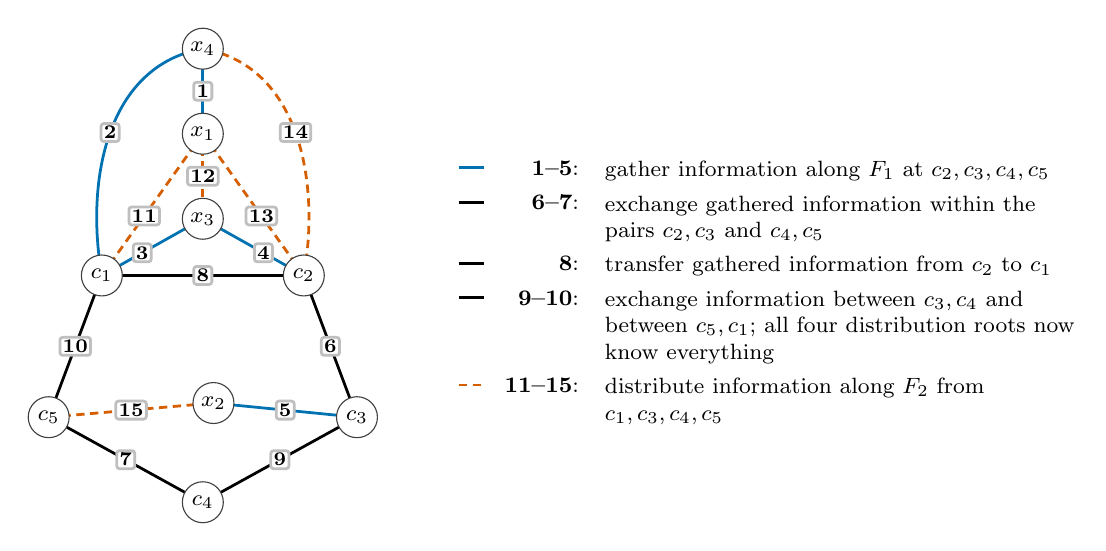
\begin{tikzpicture}[every node/.style={font=\footnotesize},
  lab/.style={fill=white,inner sep=1pt,font=\scriptsize\bfseries,rounded corners=1pt,draw=black!25,solid,text=black}]
\begin{scope}[x=1.35cm,y=1.2cm]
  \coordinate (c1) at (-0.95,0.95);
  \coordinate (c2) at (0.95,0.95);
  \coordinate (c3) at (1.45,-0.55);
  \coordinate (c4) at (0,-1.45);
  \coordinate (c5) at (-1.45,-0.55);
  \coordinate (x3) at (0,1.55);
  \coordinate (x1) at (0,2.45);
  \coordinate (x4) at (0,3.35);
  \coordinate (x2) at (0.1,-0.4);
  % cycle
  \draw[cycleedge] (c1)--(c2) node[lab,pos=.5] {8};
  \draw[cycleedge] (c2)--(c3) node[lab,pos=.5] {6};
  \draw[cycleedge] (c3)--(c4) node[lab,pos=.5] {9};
  \draw[cycleedge] (c4)--(c5) node[lab,pos=.5] {7};
  \draw[cycleedge] (c5)--(c1) node[lab,pos=.5] {10};
  % F_1 (gathering)
  \draw[blueforest] (x4)--(x1) node[lab,pos=.5] {1};
  \draw[blueforest] (x4) to[out=190,in=100] node[lab,pos=.5] {2} (c1);
  \draw[blueforest] (c1)--(x3) node[lab,pos=.4] {3};
  \draw[blueforest] (x3)--(c2) node[lab,pos=.6] {4};
  \draw[blueforest] (x2)--(c3) node[lab,pos=.5] {5};
  % F_2 (distributing)
  \draw[orangeforest] (c1)--(x1) node[lab,pos=.42] {11};
  \draw[orangeforest] (x1)--(x3) node[lab,pos=.5] {12};
  \draw[orangeforest] (x1)--(c2) node[lab,pos=.58] {13};
  \draw[orangeforest] (c2) to[out=80,in=-10] node[lab,pos=.5] {14} (x4);
  \draw[orangeforest] (c5)--(x2) node[lab,pos=.5] {15};
  \foreach \v/\l in {c1/c_1,c2/c_2,c3/c_3,c4/c_4,c5/c_5,x1/x_1,x2/x_2,x3/x_3,x4/x_4}
    \node[vertex] at (\v) {$\l$};
\end{scope}
\begin{scope}[xshift=5.1cm,yshift=2.6cm,
  desc/.style={anchor=north west,text width=60mm,align=left,inner sep=0pt,execute at begin node={\hyphenpenalty=10000\exhyphenpenalty=10000}},
  rng/.style={anchor=north east,inner sep=0pt}]
  \node[desc] (d1) at (0,0) {gather information along $F_1$ at $c_2,c_3,c_4,c_5$};
  \node[rng] (r1) at ([xshift=-9pt]d1.north west) {\textbf{1--5}:};
  \draw[blueforest] ([xshift=-1.85cm,yshift=-0.6ex]d1.north west) -- ++(0.32,0);
  \node[desc] (d2) at ([yshift=-5pt]d1.south west) {exchange gathered information within the pairs $c_2,c_3$ and $c_4,c_5$};
  \node[rng] (r2) at ([xshift=-9pt]d2.north west) {\textbf{6--7}:};
  \draw[cycleedge] ([xshift=-1.85cm,yshift=-0.6ex]d2.north west) -- ++(0.32,0);
  \node[desc] (d3) at ([yshift=-5pt]d2.south west) {transfer gathered information from $c_2$ to $c_1$};
  \node[rng] (r3) at ([xshift=-9pt]d3.north west) {\textbf{8}:};
  \draw[cycleedge] ([xshift=-1.85cm,yshift=-0.6ex]d3.north west) -- ++(0.32,0);
  \node[desc] (d4) at ([yshift=-5pt]d3.south west) {exchange information between $c_3,c_4$ and between $c_5,c_1$; all four distribution roots now know everything};
  \node[rng] (r4) at ([xshift=-9pt]d4.north west) {\textbf{9--10}:};
  \draw[cycleedge] ([xshift=-1.85cm,yshift=-0.6ex]d4.north west) -- ++(0.32,0);
  \node[desc] (d5) at ([yshift=-5pt]d4.south west) {distribute information along $F_2$ from $c_1,c_3,c_4,c_5$};
  \node[rng] (r5) at ([xshift=-9pt]d5.north west) {\textbf{11--15}:};
  \draw[orangeforest] ([xshift=-1.85cm,yshift=-0.6ex]d5.north west) -- ++(0.32,0);
\end{scope}
\end{tikzpicture}
\caption{A temporally connecting labeling of the running example from
\Cref{fig:m-graph}, obtained by the construction of
\Cref{lem:construct-labeling}. Each edge is labeled by its position in
the gossip scheme. Blue solid edges gather information at
$c_2,c_3,c_4,c_5$; black cycle edges exchange it so that the distribution
roots $c_1,c_3,c_4,c_5$ know everything after call 10; orange dashed
edges distribute it along $F_2$. Call 8 transfers information within
the only interval with more than one vertex, from $c_2$ to $c_1$.
Every edge is used exactly once.}
\label{fig:labeling-example}
\end{figure}

\section{Necessity}
\label{sec:necessity-self-contained}
We prove the necessity direction of \Cref{thm:characterization}.
Graphs with at most one vertex satisfy the characterization directly.
For a graph with at least two vertices, we construct a $T$-witness or
an $M$-witness from a complete call order. The proof has four stages.
\begin{enumerate}
\item \emph{Construct the quotient and bound its size.}
Contract maximal sets supporting two edge-disjoint spanning trees.
An exchange argument bounds the number of edges in the quotient and
gives a $T$-witness when the upper bound is attained
(\Cref{sec:necessity-blocks,sec:necessity-exchange}).
\item \emph{Establish the lifting condition.}
To lift a quotient $M$-witness, inside each block on its cycle we need
two spanning trees and a path between its attachment vertices, all
edge-disjoint. We establish a sufficient condition for finding these
subgraphs (\Cref{sec:necessity-lifting}).
\item \emph{Use the call order to obtain canonical structure.}
The call order gives a lower edge bound. At equality, it yields a
canonical division into early and future calls
(\Cref{sec:necessity-canonical}).
\item \emph{Select a compatible cycle and lift the witness.}
Use the canonical structure to select a four-cycle satisfying the
lifting condition, extend it to a quotient $M$-witness, and lift it to
the original graph
(\Cref{sec:necessity-path-selection,sec:necessity-ports}).
\end{enumerate}
\Cref{fig:necessity-roadmap} summarizes these steps and the case distinctions between them.

\begin{figure}[p]
\centering
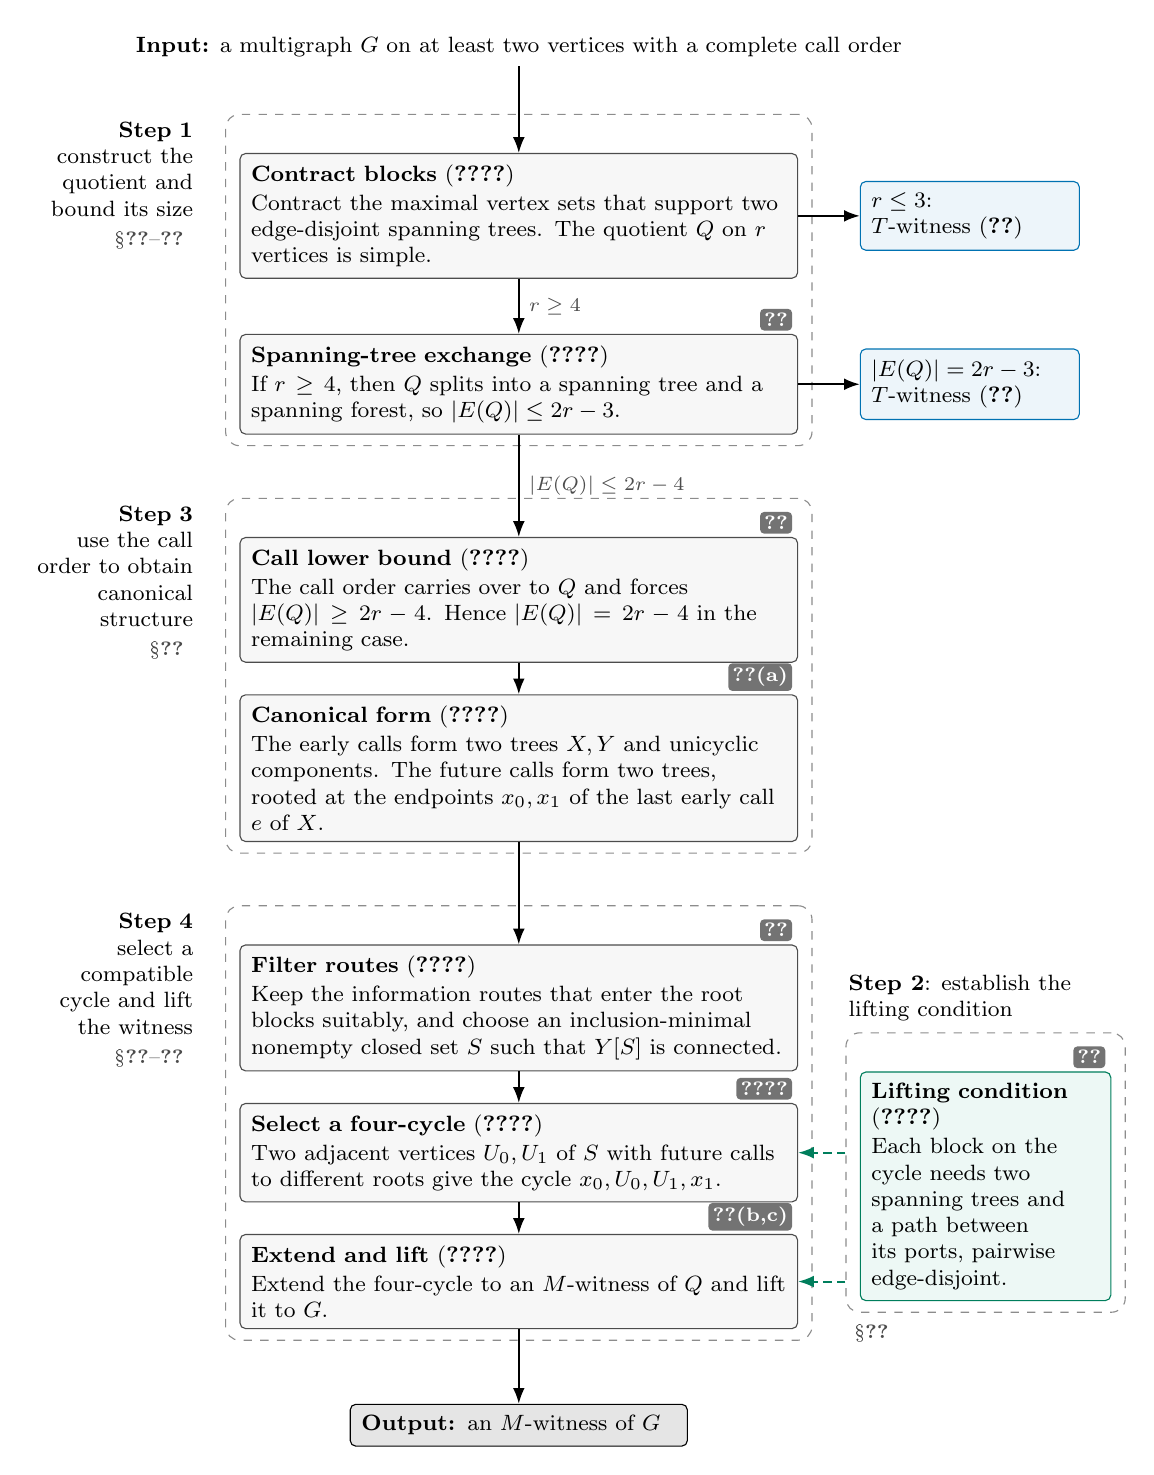
\begin{tikzpicture}[
    node distance=4mm,
    every node/.style={font=\footnotesize,execute at begin node={\hyphenpenalty=10000\exhyphenpenalty=10000}},
    stage/.style={draw=black!70,rounded corners=2pt,fill=black!3,
                  text width=68mm,inner sep=4pt,align=left},
    tool/.style={stage,text width=29mm,draw=auxgreen!80!black,fill=auxgreen!7},
    exitT/.style={draw=witnessblue,rounded corners=2pt,fill=witnessblue!7,
                  text width=25mm,inner sep=4pt,align=left},
    outbox/.style={stage,text width=40mm,draw=black,fill=black!10},
    note/.style={font=\scriptsize,text=black!70,align=left},
    figtag/.style={fill=black!55,text=white,font=\scriptsize\bfseries,
                   rounded corners=1.5pt,inner sep=1.5pt},
    arr/.style={-{Latex[length=2mm]},line width=.7pt},
    usearr/.style={-{Latex[length=2mm]},line width=.7pt,auxgreen!80!black,
                   dash pattern=on 3pt off 2pt},
    band/.style={draw=black!45,dashed,rounded corners=5pt,
                 inner xsep=5pt,inner ysep=4pt},
    steplabel/.style={anchor=north east,text width=21mm,align=right,inner sep=0pt}
]
  % ---------- input ----------
  \node (in) {\textbf{Input:} a multigraph $G$ on at least two vertices
    with a complete call order};

  % ---------- step 1 ----------
  \node[stage,below=11mm of in] (quot) {\textbf{Contract blocks}
     (\Cref{lem:characterization-union,lem:characterization-quotient})\\[1pt]
     Contract the maximal vertex sets that support two edge-disjoint
     spanning trees. The quotient $Q$ on $r$ vertices is simple.};
  \node[stage,below=7mm of quot] (exch) {\textbf{Spanning-tree exchange}
     (\Cref{lem:characterization-exchange,cor:characterization-edges})\\[1pt]
     If $r\geq4$, then $Q$ splits into a spanning tree and a spanning
     forest, so $|E(Q)|\leq2r-3$.};
  \coordinate (b1top) at ([yshift=3.5mm]quot.north);
  \node[band,fit=(quot)(exch)(b1top)] (b1) {};
  \node[steplabel] (sl1) at ([xshift=-4mm,yshift=-1mm]b1.north west) {\textbf{Step 1}\\ construct the quotient and bound its size};

  % ---------- step 3 ----------
  \node[stage,below=13mm of exch] (lower) {\textbf{Call lower bound}
     (\Cref{lem:characterization-poset-transfer,lem:characterization-closed-tree-reduction})\\[1pt]
     The call order carries over to $Q$ and forces $|E(Q)|\geq2r-4$.
     Hence $|E(Q)|=2r-4$ in the remaining case.};
  \node[stage,below=of lower] (canon) {\textbf{Canonical form}
     (\Cref{lem:characterization-canonical-ideal,cor:characterization-early-components})\\[1pt]
     The early calls form two trees $X,Y$ and unicyclic components. The
     future calls form two trees, rooted at the endpoints $x_0,x_1$ of
     the last early call $e$ of $X$.};
  \coordinate (b3top) at ([yshift=3.5mm]lower.north);
  \node[band,fit=(lower)(canon)(b3top)] (b3) {};
  \node[steplabel] (sl3) at ([xshift=-4mm,yshift=-1mm]b3.north west) {\textbf{Step 3}\\ use the call order to obtain canonical structure};

  % ---------- step 4 ----------
  \node[stage,below=13mm of canon] (filter) {\textbf{Filter routes}
     (\Cref{lem:characterization-root-good-routes,lem:characterization-actual-closed-set})\\[1pt]
     Keep the information routes that enter the root blocks suitably,
     and choose an inclusion-minimal nonempty closed set $S$ such that
     $Y[S]$ is connected.};
  \node[stage,below=of filter] (select) {\textbf{Select a four-cycle}
     (\Cref{lem:characterization-same-index-rerouting,lem:characterization-compatible-actual-cycle})\\[1pt]
     Two adjacent vertices $U_0,U_1$ of $S$ with future calls to
     different roots give the cycle $x_0,U_0,U_1,x_1$.};
  \node[stage,below=of select] (extend) {\textbf{Extend and lift}
     (\Cref{lem:characterization-protected-extension,cor:characterization-optimal-quotient-lift})\\[1pt]
     Extend the four-cycle to an $M$-witness of $Q$ and lift it to $G$.};
  \coordinate (b4top) at ([yshift=3.5mm]filter.north);
  \node[band,fit=(filter)(select)(extend)(b4top)] (b4) {};
  \node[steplabel] (sl4) at ([xshift=-4mm,yshift=-1mm]b4.north west) {\textbf{Step 4}\\ select a compatible cycle and lift the witness};

  % ---------- step 2 (tool) ----------
  \node[tool,anchor=north west] (lift) at ([xshift=6mm]b4.east|-filter.south)
     {\textbf{Lifting condition}\\
     (\Cref{lem:characterization-m-lift,lem:characterization-threshold})\\[1pt]
     Each block on the cycle needs two spanning trees and a path between
     its ports, pairwise edge-disjoint.};
  \coordinate (b2top) at ([yshift=3.5mm]lift.north);
  \node[band,fit=(lift)(b2top)] (b2) {};
  \node[font=\footnotesize,anchor=south west,inner sep=1pt,align=left] (sl2) at ([yshift=1mm]b2.north west) {\textbf{Step 2}: establish the\\ lifting condition};

  % ---------- exits ----------
  \node[exitT,anchor=west] (t1) at ([xshift=6mm]b1.east|-quot) {$r\leq3$:\\ $T$-witness
     (\Cref{lem:characterization-t-lift})};
  \node[exitT,anchor=west] (t2) at ([xshift=6mm]b1.east|-exch) {$|E(Q)|=2r-3$:\\ $T$-witness
     (\Cref{cor:characterization-t-case})};
  \node[outbox,below=8mm of b4.south] (outM) {\textbf{Output:} an $M$-witness of $G$};

  % ---------- arrows ----------
  \draw[arr] (in)--(quot);
  \draw[arr] (quot)--node[right,note]{$r\geq4$}(exch);
  \draw[arr] (quot.east)--(t1.west);
  \draw[arr] (exch.east)--(t2.west);
  \draw[arr] (exch.south)--node[right,note]{$|E(Q)|\leq2r-4$}(lower.north);
  \draw[arr] (lower)--(canon);
  \draw[arr] (canon.south)--(filter.north);
  \draw[arr] (filter)--(select);
  \draw[arr] (select)--(extend);
  \draw[arr] (extend.south)--(outM.north);
  \draw[usearr] (b2.west|-select)--(select.east);
  \draw[usearr] (b2.west|-extend)--(extend.east);

  % ---------- figure tags ----------
  \node[figtag,anchor=south east] at ([xshift=-2pt,yshift=1pt]exch.north east) {\Cref{fig:exchange}};
  \node[figtag,anchor=south east] at ([xshift=-2pt,yshift=1pt]lower.north east) {\Cref{fig:closed-tree}};
  \node[figtag,anchor=south east] at ([xshift=-2pt,yshift=1pt]canon.north east) {\Cref{fig:necessity-canonical}(a)};
  \node[figtag,anchor=south east] at ([xshift=-2pt,yshift=1pt]filter.north east) {\Cref{fig:filtered-routes}};
  \node[figtag,anchor=south east] at ([xshift=-2pt,yshift=1pt]select.north east) {\Cref{fig:static-selection,fig:port-selection}};
  \node[figtag,anchor=south east] at ([xshift=-2pt,yshift=1pt]extend.north east) {\Cref{fig:necessity-canonical}(b,c)};
  \node[figtag,anchor=south east] at ([xshift=-2pt,yshift=1pt]lift.north east) {\Cref{fig:nonliftable}};

  % ---------- section column ----------
  \foreach \b/\s in {1/{\S\ref{sec:necessity-blocks}--\ref{sec:necessity-exchange}},
                     3/{\S\ref{sec:necessity-canonical}},
                     4/{\S\ref{sec:necessity-path-selection}--\ref{sec:necessity-ports}}}
    \node[note,anchor=north east,align=right] at ([yshift=-2pt]sl\b.south east) {\s};
  \node[note,anchor=north west] at ([yshift=-1pt]b2.south west) {\S\ref{sec:necessity-lifting}};
\end{tikzpicture}
\caption{Roadmap of the necessity proof of \Cref{thm:characterization}.
The dashed boxes are the four steps listed at the beginning of
\Cref{sec:necessity-self-contained}. Small quotients and the upper edge
count give a $T$-witness (blue). Otherwise, the call order fixes the
edge count and the canonical structure, which guides the choice of a
four-cycle that satisfies the lifting condition of Step~2 (green, dashed
arrows). The gray tags name the figures illustrating each part.}
\label{fig:necessity-roadmap}
\end{figure}


\subsection{Two-Tree Blocks and Their Quotient}
\label{sec:necessity-blocks}
We first construct the quotient and show that its $T$-witnesses lift
to the original graph. Fix a multigraph $G$ with a complete call
order. Within this argument graphs are loopless: deleting loops
preserves completeness, since they transmit no new secret. Paths may
be trivial, and spanning subgraphs retain isolated vertices. For an
edge set $A$, the notation $H[A]$ denotes the spanning subgraph with
edge set $A$; for a vertex set it denotes the induced subgraph.
Deleting a path means deleting its edges. A path is \emph{nonseparating}
if this deletion leaves its ambient graph connected.

In a graph $H$, a nonempty vertex set $X\subseteq V(H)$ is a
\emph{two-tree set} if $H[X]$ contains two edge-disjoint spanning trees.
It is \emph{nontrivial} if $|X|\geq2$. A singleton is a two-tree set,
with two empty trees. These are the vertex sets of the $T^*$-subgraphs of
Burosch and Laborde~\cite{BuroschL92}.

\begin{lemma}\label{lem:characterization-union}
If $X$ and $Y$ are two-tree sets and $X\cap Y\neq\varnothing$, then
$X\cup Y$ is a two-tree set.
\end{lemma}
\begin{proof}
Choose edge-disjoint spanning trees $A_X,B_X$ of $G[X]$ and
$A_Y,B_Y$ of $G[Y]$. The graph with edge set $E(A_X)\cup E(A_Y)$
is connected on $X\cup Y$. Extend $A_X$ to a spanning tree $A$ of
this graph. Every edge of $A$ outside $A_X$ belongs to $A_Y$ and has
at least one endpoint outside $X$: otherwise it would form a cycle
with the spanning tree $A_X$ on $X$.

Consider the graph on $X\cup Y$ with edge set
\[
 E(B_X)\cup\bigl(E(B_Y)\setminus E(A_X)\bigr).
\]
It is edge-disjoint from $A$. Indeed, $B_X$ avoids $A_X$, and its
edges have both endpoints in $X$, so it also avoids $A-A_X$.
The retained edges of $B_Y$ avoid $A_X$ by definition and avoid
$A-A_X$ because the latter edges belong to $A_Y$.
The graph is connected: every deleted edge of $B_Y$ belongs to $A_X$
and has both endpoints in $X\cap Y$, so its endpoints can instead
be joined through $B_X$. Thus it contains a spanning tree $B$
edge-disjoint from $A$.
\end{proof}

We use this union property to decompose the graph into maximal
two-tree sets.

\begin{corollary}\label{cor:characterization-partition}
The inclusion-maximal two-tree sets form a partition $\mathcal B$ of
$V(G)$.
\end{corollary}
\begin{proof}
Every vertex belongs to a two-tree set and hence, by finiteness, to a
maximal one. Two distinct maximal sets cannot intersect by
\Cref{lem:characterization-union}.
\end{proof}

We call the sets in $\mathcal B$ \emph{blocks}. Let $Q$ be obtained by
contracting each block to one vertex. Delete edges internal to a block, and retain each external edge
as a distinct edge of $Q$, together with its original endpoints.

\begin{lemma}\label{lem:characterization-quotient}
The quotient $Q$ is simple and contains no nontrivial two-tree set. If $G$ is connected, then $Q$ is connected.
\end{lemma}
\begin{proof}
The quotient $Q$ has no loops, since all edges internal to a block
were deleted. Suppose a set of at least two vertices of $Q$ supports
two edge-disjoint spanning trees. Lift their edges to $G$. In each
represented block, add one internal spanning tree to the first lift
and the other to the second. Each lift is connected and has exactly
one less edge than vertices, so the two lifts are edge-disjoint
spanning trees on the union of the blocks. This contradicts their
maximality. Two parallel edges of $Q$ would themselves be two
edge-disjoint spanning trees on their two endpoints, so no parallel
edges occur. Connectivity is preserved by contracting connected sets.
\end{proof}

A $T$-witness of the quotient lifts to the original graph by using
the two internal spanning trees in each block.

\begin{lemma}\label{lem:characterization-t-lift}
If $Q$ has a $T$-witness, then $G$ has a $T$-witness. If $Q$ has one
vertex, then $G$ has two edge-disjoint spanning trees.
\end{lemma}
\begin{proof}
Lift each quotient tree and add one of the two internal spanning trees
in every block. The two resulting graphs are spanning trees, and their
intersection consists precisely of the lifts of shared quotient edges.
The one-vertex case is the definition of a two-tree block.
\end{proof}

\subsection{Spanning-Tree Exchange}
\label{sec:necessity-exchange}

The following lemma lets us replace a chosen spanning tree so that
the remaining edges form a forest, without losing connections already
present in the complement. Components of the complement may merge,
but none split. This lets us bound the quotient's edge count and later
modify trees while preserving specified complementary components.
The lemma is adapted from Burosch and
Laborde~\cite[Lemma~3]{BuroschL92}. A partition \emph{coarsens}
another if every part of the latter is contained in a part of the former.

\begin{figure}[t]
\centering
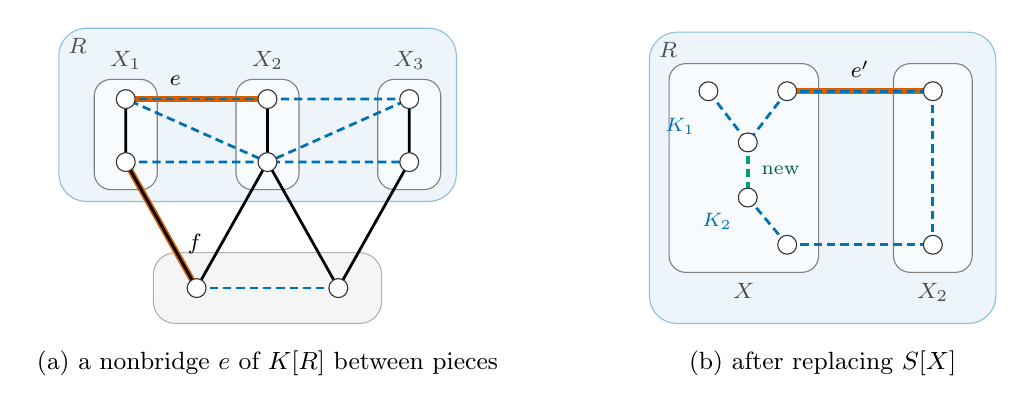
\begin{tikzpicture}[
  every node/.style={font=\footnotesize},
  v/.style={circle,draw=black!80,fill=white,inner sep=0pt,minimum size=2.4mm},
  sE/.style={black,line width=1pt},
  kE/.style={witnessblue,line width=1pt,dash pattern=on 3pt off 1.8pt},
  hlE/.style={witnessorange,line width=2.2pt},
  newE/.style={auxgreen,line width=1.4pt,dash pattern=on 3pt off 1.8pt},
  regionR/.style={fill=witnessblue!7,draw=witnessblue!45,rounded corners=10pt},
  regionO/.style={fill=black!4,draw=black!30,rounded corners=8pt},
  piece/.style={draw=black!50,rounded corners=6pt,fill=white,fill opacity=.6},
  lbl/.style={font=\footnotesize,text=black!70},
]
% ================= panel (a) =================
\begin{scope}
  \draw[regionR] (-0.85,-0.4) rectangle (4.2,1.8);
  \node[lbl,anchor=north west] at (-0.85,1.8) {$R$};
  \draw[regionO] (0.35,-1.95) rectangle (3.25,-1.05);
  \foreach \i/\x in {1/0,2/1.8,3/3.6} {
    \draw[piece] (\x-0.4,-0.25) rectangle (\x+0.4,1.15);
    \node[lbl,anchor=south] at (\x,1.15) {$X_\i$};}
  \coordinate (u1) at (0,0.9);   \coordinate (u2) at (0,0.1);
  \coordinate (v1) at (1.8,0.9); \coordinate (v2) at (1.8,0.1);
  \coordinate (w1) at (3.6,0.9); \coordinate (w2) at (3.6,0.1);
  \coordinate (o1) at (0.9,-1.5); \coordinate (o2) at (2.7,-1.5);
  % complement K
  \draw[kE] (o1)--(o2);
  \draw[kE] (v1)--(w1)--(v2)--(u1) (u2)--(v2)--(w2);
  \draw[hlE] (u1)--(v1);
  \draw[kE] (u1)--(v1) node[pos=.35,above=1pt,text=black] {$e$};
  % spanning tree S
  \draw[sE] (u1)--(u2) (v1)--(v2) (w1)--(w2) (o1)--(v2)--(o2)--(w2);
  \draw[hlE] (u2)--(o1);
  \draw[sE] (u2)--(o1) node[pos=.65,right=2pt,text=black] {$f$};
  \foreach \p in {u1,u2,v1,v2,w1,w2,o1,o2} \node[v] at (\p) {};
  \node[panel] at (1.8,-2.45) {(a) a nonbridge $e$ of $K[R]$ between pieces};
\end{scope}
% ================= panel (b) =================
\begin{scope}[xshift=7.4cm]
  \draw[regionR] (-0.75,-1.95) rectangle (3.65,1.75);
  \node[lbl,anchor=north west] at (-0.75,1.75) {$R$};
  \draw[piece] (-0.5,-1.3) rectangle (1.4,1.35);  \node[lbl,anchor=north] at (0.45,-1.32) {$X$};
  \draw[piece] (2.35,-1.3) rectangle (3.35,1.35); \node[lbl,anchor=north] at (2.85,-1.32) {$X_2$};
  \coordinate (a1) at (0,1.0); \coordinate (a2) at (1.0,1.0); \coordinate (a3) at (0.5,0.35);
  \coordinate (b1) at (0.5,-0.35); \coordinate (b2) at (1.0,-0.95);
  \coordinate (y1) at (2.85,1.0); \coordinate (y2) at (2.85,-0.95);
  \draw[kE] (a2)--(a3)--(a1);
  \draw[kE] (b1)--(b2);
  \draw[kE] (y1)--(y2);
  \draw[hlE] (a2)--(y1);
  \draw[kE] (a2)--(y1) node[midway,above=1pt,text=black] {$e'$};
  \draw[kE] (b2)--(y2);
  \draw[newE] (a3)--(b1) node[midway,right=1pt,font=\scriptsize,text=auxgreen!60!black] {new};
  \foreach \p in {a1,a2,a3,b1,b2,y1,y2} \node[v] at (\p) {};
  \node[font=\scriptsize,text=witnessblue,anchor=east] at (-0.05,0.55) {$K_1$};
  \node[font=\scriptsize,text=witnessblue,anchor=east] at (0.42,-0.65) {$K_2$};
  \node[panel] at (1.45,-2.45) {(b) after replacing $S[X]$};
\end{scope}
\end{tikzpicture}
\caption{The two steps in the proof of \Cref{lem:characterization-exchange}.
Black edges belong to the spanning tree $S$, and blue dashed edges to its
complement $K$. For a component $R$ of $K$ (blue region), the boxes are
the vertex sets $X_i$ of the components of $S[R]$.
(a) If a complementary edge $e$ joining two pieces were not a bridge of
$K[R]$, the $S$-path between its endpoints would leave $R$ through an
edge $f$. Exchanging $e$ and $f$ keeps $K[R]-e$ connected and joins $R$ to
another component of the complement, reducing the number of components.
(b) If $K[R]$ contains a cycle, it lies in one piece $X$, here in the
component $K_1$ of $K[X]$. Replacing $S[X]$ by induction makes the
complement inside $X$ a forest that keeps every component of $K[X]$
connected and joins two of them. Here, the replacement removes a cycle
edge inside $K_1$ and adds the green connection between $K_1$ and $K_2$.
The old path between them leaves $X$ through a bridge $e'$ between
pieces, which now lies on a cycle of the complement. The same argument is used in
\Cref{lem:characterization-protected-extension}.}
\label{fig:exchange}
\end{figure}

\begin{lemma}\label{lem:characterization-exchange}
Let $H$ be connected and loopless, with no nontrivial two-tree set.
For every spanning tree $T$ of $H$, there is a spanning tree $S$ such
that $H-E(S)$ is a forest and its component partition coarsens that
of $H-E(T)$.
\end{lemma}

We choose a spanning tree whose complement has as few components as
possible, subject to the coarsening condition. If the complement
contains a cycle, we modify the tree inside that component using
induction. The modified tree admits an exchange that reduces the
number of complementary components, contradicting minimality.
\Cref{fig:exchange} illustrates both steps.

\begin{proof}[Proof of \Cref{lem:characterization-exchange}]
Induct on $|V(H)|$. The assertion is immediate for one vertex.
Among the spanning trees satisfying the required coarsening condition,
choose $S$ so that $H-E(S)$ has as few components as possible. Such a
tree exists because $T$ satisfies the condition. Write $K=H-E(S)$.

Fix a component of $K$ with vertex set $R$, and let $X_1,\ldots,X_s$
be the vertex sets of the components of $S[R]$.
Every edge $e$ of $K[R]$ joining different sets $X_i$ is a bridge
of $K[R]$. Otherwise, the unique $S$-path between its endpoints must
leave $R$, since its endpoints are in different components of $S[R]$.
Choose an edge $f$ of this path with one endpoint in $R$ and the other
outside $R$. Replacing $f$ by $e$ in $S$ gives another spanning tree.
Deleting $e$ from $K[R]$ does not disconnect it, whereas adding $f$
joins it to another component of $K$. The new complementary partition
therefore coarsens that of $K$ and has fewer components, a contradiction.
This bridge property holds for every minimizing tree $S$.

Suppose now that $K[R]$ contains a cycle. Since $H$ is loopless,
$|R|\geq2$. None of its edges is a
bridge, so the cycle lies entirely inside one of the sets $X_i$;
call that set $X$. If $s=1$, then $S[R]$ and a spanning
tree of $K[R]$ would be two edge-disjoint spanning trees on $R$, contrary
to the hypothesis. Hence $s\geq2$, and in particular
$|X|<|V(H)|$.

Apply the inductive hypothesis to the connected induced graph $H[X]$
and its spanning tree $S[X]$. Obtain a spanning tree $S_X$ whose
complement is a forest and whose complementary partition coarsens
that of $K[X]$. Replace $S[X]$ in $S$ by $S_X$, obtaining a spanning
tree $\widetilde S$ of $H$. Its complementary partition is exactly
that of $K$. Indeed, each old component of $K[X]$ remains connected,
all edges outside $H[X]$ are retained, and all newly added complementary
edges have endpoints in $R$; thus no old component splits or merges
with a different old component. Moreover, the component vertex sets
of $\widetilde S[R]$ are still $X_1,\ldots,X_s$.

Let $q$ be the number of components of $K[X]$. Since it contains a
cycle, it has at least $|X|-q+1$ edges. The new complement in $H[X]$
has the same number of edges, because both replaced trees have
$|X|-1$ edges. Being a forest, it therefore has at most $q-1$
components. Consequently, it connects two distinct old components
of $K[X]$.

Choose vertices in these two old components and a simple path between
them in $K[R]$. This path must leave $X$. It thus contains an edge $e$
joining different sets $X_i$, which is a bridge of $K[R]$ by the
bridge property. Removing $e$ separates the two selected vertices.
Every component of $K[X]$ lies on one side of this cut, and its
vertices remain connected after the replacement. The edges outside
$H[X]$, other than $e$, are unchanged. Hence the old connections on
each side of the cut remain, while the new connection inside $X$
joins the two sides without using $e$. The edge $e$ is consequently
not a bridge of $H-E(\widetilde S)$.
But $\widetilde S$ is also a minimizing tree, and $e$ still joins
different components of $\widetilde S[R]$. This contradicts the
bridge property. Thus $K$ is a forest.
\end{proof}

The partition into a spanning tree and a complementary forest bounds
the number of edges.

\begin{corollary}\label{cor:characterization-edges}
If $H$ is connected and loopless, has $r\geq2$ vertices, and contains
no nontrivial two-tree set, then $|E(H)|\leq2r-3$.
\end{corollary}
\begin{proof}
By \Cref{lem:characterization-exchange}, the edges partition into a spanning
tree and a spanning forest. The forest has at least two components,
since otherwise $H$ itself would be a two-tree set. The two parts
have at most $r-1$ and $r-2$ edges, respectively.
\end{proof}

When the quotient attains this bound, the complementary forest has
exactly two components, which yields a $T$-witness.

\begin{corollary}\label{cor:characterization-t-case}
If the connected quotient $Q$ has $r\geq2$ vertices and $2r-3$ edges,
then $G$ has a $T$-witness.
\end{corollary}
\begin{proof}
The partition supplied by \Cref{lem:characterization-exchange} consists of a
spanning tree $A$ and a spanning forest $B$ with exactly two components.
Choose an edge $e$ of $A$ joining these components. The trees $A$
and $B+e$ share exactly $e$. Apply \Cref{lem:characterization-t-lift}.
\end{proof}

\subsection{Lifting Witnesses}
\label{sec:necessity-lifting}

Two internal spanning trees suffice to lift a quotient $T$-witness.
For a quotient cycle, those same two trees may leave no internal
path between its attachment vertices. The next lemma isolates the
additional condition needed for lifting.

\begin{lemma}\label{lem:characterization-m-lift}
Suppose $Q$ has an $M$-witness $(D,L_1,L_2)$. For each block $X$
represented on $D$, let $p_X,q_X$ be the original endpoints in $X$
of its two incident cycle edges. Suppose $G[X]$ has two spanning
trees $A_X,B_X$ and a $p_X$-$q_X$ path $P_X$ whose three edge sets
are pairwise disjoint. Then $G$ has an $M$-witness.
\end{lemma}
\begin{proof}
In blocks off $D$, choose any two edge-disjoint internal spanning
trees and call them $A_X,B_X$ as well. Lift $L_1,L_2$ and add all
trees $A_X,B_X$, respectively. Replacing each quotient vertex by an
internal tree preserves the component partition. A cycle in the lift
could not lie inside one block, whose internal edges form a tree.
Its external edges would therefore project to a nonempty closed trail
in the quotient forest, which is impossible. Thus each lift is a
forest with exactly four components.
The two lifted forests are edge-disjoint: their external edges come
from the edge-disjoint quotient forests $L_1,L_2$, and their internal edges
come from the edge-disjoint trees $A_X,B_X$ in each block.
Replace each vertex $X$ on $D$ by $P_X$. Paths in different blocks
are vertex-disjoint, and each block occurs only once on $D$, so this
gives a cycle of length at least four. A path may be trivial if
$p_X=q_X$. The lifted cycle avoids both forests by the local
edge-disjointness assumptions and the edge-disjointness of the quotient
witness. Every forest component still meets the lifted cycle.
\end{proof}

To obtain the local condition in \Cref{lem:characterization-m-lift}, we will find
a nonseparating path on one side of a call threshold and a spanning
tree on the other side. The two threshold graphs have disjoint edges.

\begin{lemma}\label{lem:characterization-threshold}
Let $J$ be a graph and let $E^-,E^+\subseteq E(J)$ be disjoint.
Suppose $(V(J),E^+)$ is connected and there is a $p$-$q$ path
$P$ in $(V(J),E^-)$ such that $(V(J),E^-\setminus E(P))$ is
connected. Then $J$ contains two spanning trees and a $p$-$q$
path whose edge sets are pairwise disjoint.
\end{lemma}
\begin{proof}
Choose one spanning tree from $E^-\setminus E(P)$ and another
from $E^+$. Both avoid $P$, and they avoid each other.
\end{proof}

Finding an $M$-witness in the quotient is not sufficient: its cycle
may fail to lift while remaining edge-disjoint from the two forests.
The following example explains why we must also control the cycle's
attachment vertices inside each block. Consider the
five-cycle $(a,x,b,c,d,a)$ and add a second copy of the edge $ax$.
The set $\{a,x\}$ is a two-tree block, and contracting it produces a
four-cycle. The original graph has no $T$-witness: two spanning trees
sharing at most one edge require at least seven edges, but it has six.
It also has no $M$-witness: its only cycles of length at least four
have length five, leaving just one edge for two forests that would
each need one edge. Thus an $M$-witness of the quotient need not lift (\Cref{fig:nonliftable}).
The two internal edges of the block cannot supply both two spanning
trees and a path from $a$ to $x$.

\begin{figure}[t]
\centering
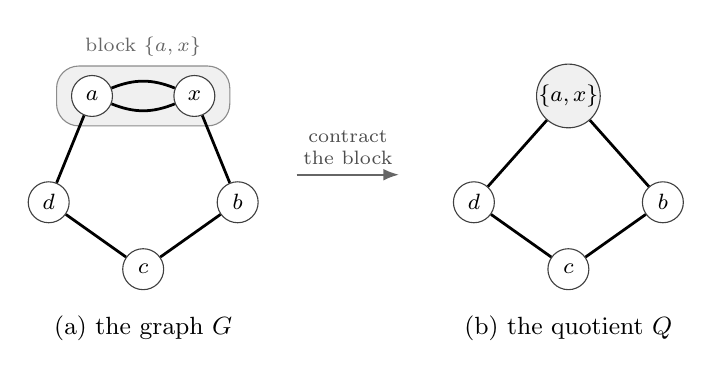
\begin{tikzpicture}[
  every node/.style={font=\footnotesize},
  blk/.style={rounded corners=8pt,draw=black!45,fill=black!6},
  arr/.style={-{Latex[length=2mm]},line width=.8pt,black!60},
]
\begin{scope}
  \draw[blk] (-0.45,0.62) rectangle (1.75,1.38);
  \node[vertex] (a) at (0,1) {$a$};
  \node[vertex] (x) at (1.3,1) {$x$};
  \node[vertex] (b) at (1.85,-0.35) {$b$};
  \node[vertex] (c) at (0.65,-1.2) {$c$};
  \node[vertex] (d) at (-0.55,-0.35) {$d$};
  \draw[cycleedge] (a) to[bend left=22] (x);
  \draw[cycleedge] (a) to[bend right=22] (x);
  \draw[cycleedge] (x)--(b)--(c)--(d)--(a);
  \node[font=\scriptsize,text=black!60,anchor=south] at (0.65,1.38) {block $\{a,x\}$};
  \node[panel] at (0.65,-1.95) {(a) the graph $G$};
\end{scope}
\draw[arr] (2.6,0)--node[above,font=\scriptsize,text=black!70,align=center]{contract\\the block}(3.9,0);
\begin{scope}[xshift=5.4cm]
  \node[vertex,fill=black!6,minimum size=6mm] (ax) at (0.65,1) {$\{a,x\}$};
  \node[vertex] (b) at (1.85,-0.35) {$b$};
  \node[vertex] (c) at (0.65,-1.2) {$c$};
  \node[vertex] (d) at (-0.55,-0.35) {$d$};
  \draw[cycleedge] (ax)--(b)--(c)--(d)--(ax);
  \node[panel] at (0.65,-1.95) {(b) the quotient $Q$};
\end{scope}
\end{tikzpicture}
\caption{A quotient $M$-witness that does not lift. (a) The graph $G$ has
six edges on five vertices, so it has no $T$-witness. Its only cycles of
length at least four have length five, leaving one edge for two forests,
so it has no $M$-witness either. (b) The quotient $Q$ is a four-cycle,
which is an $M$-witness with empty forests. The two internal edges of the
block cannot supply both two spanning trees and an $a$-$x$ path. A third internal spanning tree, edge-disjoint from the first two,
would supply such a path.}
\label{fig:nonliftable}
\end{figure}

\subsection{Causal Orders and Canonical Form}
\label{sec:necessity-canonical}
We now use the complete call order to establish a lower bound on the
quotient's number of edges and describe its structure when this bound
is attained. Rather than fix one chronological order, we retain the
comparisons between calls that preserve information propagation.
This allows us to rearrange calls while keeping the scheme complete.
We first define this partial order on the original calls and then
restrict it to the quotient calls, so that the later lifting argument
retains access to paths inside the original blocks.

For a partial order, an \emph{ideal} is a set closed under
predecessors. A comparison $a<b$ is a \emph{cover} if no element lies
strictly between $a,b$. A \emph{linear extension} is a total order
respecting every comparison. We write $a<S$ when $a<s$ for every
$s\in S$.

Fix a complete call order of $G$. Its \emph{causal order} $P$ is the
transitive closure of the relations $a<b$ between chronologically
ordered calls sharing an original endpoint. A linear extension of $P$
preserves every information path and hence remains complete. Let $P_Q$
be the restriction to the external calls, identified with $E(Q)$.

\begin{lemma}\label{lem:characterization-poset-transfer}
Every linear extension of $P_Q$ is complete on $Q$.
Every cover of $P_Q$ relates incident edges of $Q$.
\end{lemma}
\begin{proof}
For any ordered pair of quotient vertices, choose an original vertex
in each corresponding block and an increasing information path
between them. Project this path to $Q$, omitting internal calls.
The retained external calls increase in $P_Q$.
Removing closed subwalks preserves this property. Thus $P_Q$ is
admissible: it provides an increasing path between every ordered pair
of quotient vertices. Every linear extension preserves these paths.

For a cover $a<_{P_Q}b$, take an original causal chain from $a$ to
$b$. It has no intermediate external call, since that would lie
strictly between $a$ and $b$ in $P_Q$. Its intermediate internal calls
all belong to one block: successive calls sharing an original endpoint
cannot move between blocks without an external call. Therefore $a,b$
share that block in $Q$. The same conclusion holds for a chain with
no intermediate call.
\end{proof}

This order must not be replaced by the usual causal order obtained by
treating every quotient block as one vertex. Such a replacement would
add comparisons between calls using different original attachment
vertices, without providing internal paths between those vertices.

\subsubsection{Closed-Tree Normalization and Counting}

By \Cref{cor:characterization-edges}, a quotient on $r\geq4$ vertices
has at most $2r-3$ edges. We now show that completeness requires at
least $2r-4$ edges. The case of $2r-3$ edges already yields a
$T$-witness by \Cref{cor:characterization-t-case}, so only the case of
$2r-4$ edges remains for the subsequent $M$-witness construction.
We rearrange the early calls
to obtain a closed tree component. If this component is nontrivial,
each of its maximal calls precedes every future call. Placing one
such call last among the early calls lets us count distinct first
future calls at all vertices except its two endpoints. A singleton
component gives a separate, stronger bound. The closedness condition
below enables the exchanges needed to obtain this division.

Let $H$ be a finite simple graph on $r\ge4$ vertices, with a partial
order $P$ whose covers relate incident edges and whose linear
extensions are complete. The ideal-exchange argument follows
Bumby~\cite{Bumby81} and Kleitman and Shearer~\cite{KleitmanS80}.
Relative to an ideal $J$, we call its edges early calls and the
remaining edges future calls. A linear extension placing $J$ first
realizes this division chronologically.

A tree component $A$ of an ideal $J$ is
\emph{closed} if there is no ideal $J'\supsetneq J$ such that
$V(A)$ is the vertex set of a component of $H[J']$ and
$(J'\setminus J)\cap E(H[V(A)])\neq\varnothing$. Thus no larger
ideal can add an internal edge while retaining this component's vertex set.

The following elementary observations will be used throughout.
\begin{enumerate}
\item A tree component is closed precisely when no minimal edge outside
$J$ is internal to it. Indeed, an internal minimal edge can be added;
conversely, a saturated predecessor chain among the edges added by
any larger ideal cannot move from an internal edge to an entirely
outside edge, since covers are adjacent.
\item An edge maximal in a
component of $H[J]$ is maximal in $J$, since a saturated chain in $J$
cannot leave that component.
\item For a maximal edge $a\in J$ and a
minimal edge $b\notin J$, a comparison $a<b$ is a cover; if they
are incomparable, $(J\setminus\{a\})\cup\{b\}$ is an ideal.
\item Closure persists
under enlargement of the ideal while the component is retained.
\end{enumerate}

If an ideal has two tree components, exchanges preserving its size
produce an ideal with a closed tree component. To see this, take two
tree components $A,B$. If neither is closed, choose a minimal
remaining internal edge $b$ of $B$ and a maximal edge $a$ of $A$.
The two edges are incomparable: the reverse comparison contradicts
ideality, whereas $a<b$ would be an adjacent cover between disjoint
components. Swapping $a,b$ splits $A$ into two trees and makes $B$
cyclic. Repeat with the two pieces of $A$. Their total vertex count
is strictly smaller than $|V(A)|+|V(B)|$, so induction terminates. A
singleton component is already closed.

\begin{figure}[t]
\centering
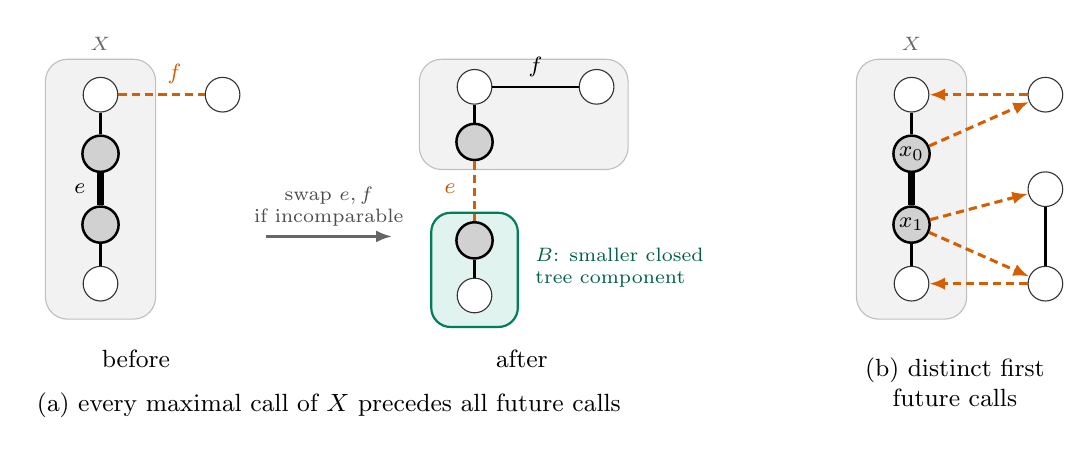
\begin{tikzpicture}[
  every node/.style={font=\footnotesize},
  v/.style={circle,draw=black!80,fill=white,inner sep=0pt,minimum size=4.4mm},
  rv/.style={circle,draw=black,fill=black!18,line width=.9pt,inner sep=0pt,minimum size=4.6mm},
  early/.style={black,line width=.9pt},
  lastcall/.style={black,line width=2.4pt},
  futE/.style={witnessorange,line width=1pt,dash pattern=on 3pt off 1.8pt},
  firstE/.style={witnessorange,line width=1.1pt,dash pattern=on 3pt off 1.8pt,
                 -{Latex[length=2mm,width=1.6mm]}},
  comp/.style={rounded corners=8pt,fill=black!5,draw=black!25},
  newB/.style={rounded corners=7pt,fill=auxgreen!12,draw=auxgreen!80!black,line width=.8pt},
  arr/.style={-{Latex[length=2mm]},line width=.8pt,black!60},
  lbl/.style={font=\scriptsize,text=black!60},
]
% ================= panel (a): the exchange =================
\begin{scope}
  \draw[comp] (-0.4,-1.65) rectangle (1.0,1.65);
  \node[lbl] at (0.3,1.85) {$X$};
  \node[rv] (x0) at (0.3,0.45) {};  \node[rv] (x1) at (0.3,-0.45) {};
  \node[v] (t1) at (0.3,1.2) {};    \node[v] (t2) at (0.3,-1.2) {};
  \node[v] (o) at (1.85,1.2) {};
  \draw[early] (t1)--(x0) (x1)--(t2);
  \draw[lastcall] (x0)--(x1) node[midway,left=1pt] {$e$};
  \draw[futE] (t1)--(o) node[pos=.65,above] {$f$};
  \node[panel] at (0.75,-2.15) {before};
\end{scope}
\draw[arr] (2.4,-0.6)--node[above,font=\scriptsize,text=black!70,align=center]{swap $e,f$\\if incomparable}(4.0,-0.6);
\begin{scope}[xshift=4.75cm]
  \draw[comp] (-0.4,0.25) rectangle (2.25,1.65);
  \draw[newB] (-0.25,-1.75) rectangle (0.85,-0.3);
  \node[font=\scriptsize,text=auxgreen!60!black,anchor=west,align=left] at (0.95,-1.0) {$B$: smaller closed\\ tree component};
  \node[rv] (x0) at (0.3,0.6) {};  \node[rv] (x1) at (0.3,-0.65) {};
  \node[v] (t1) at (0.3,1.3) {};    \node[v] (t2) at (0.3,-1.35) {};
  \node[v] (o) at (1.85,1.3) {};
  \draw[early] (t1)--(x0) (x1)--(t2) (t1)--(o) node[midway,above] {$f$};
  \draw[futE,line width=1.3pt] (x0)--(x1);
  \node[anchor=east,inner sep=1.5pt,fill=white,text=witnessorange!90!black] at (0.12,0.0) {$e$};
  \node[panel] at (0.9,-2.15) {after};
\end{scope}
\node[panel] at (3.2,-2.75) {(a) every maximal call of $X$ precedes all future calls};
% ================= panel (b): first future calls =================
\begin{scope}[xshift=10.3cm]
  \draw[comp] (-0.4,-1.65) rectangle (1.0,1.65);
  \node[lbl] at (0.3,1.85) {$X$};
  \node[rv] (x0) at (0.3,0.45) {$x_0$};  \node[rv] (x1) at (0.3,-0.45) {$x_1$};
  \node[v] (t1) at (0.3,1.2) {};    \node[v] (t2) at (0.3,-1.2) {};
  \draw[early] (t1)--(x0) (x1)--(t2);
  \draw[lastcall] (x0)--(x1);
  \node[v] (o1) at (2.0,1.2) {};
  \node[v] (o2) at (2.0,0.0) {};
  \node[v] (o3) at (2.0,-1.2) {};
  \draw[early] (o2)--(o3);
  \draw[firstE] (x0)--(o1);
  \draw[firstE] (o1)--(t1);
  \draw[firstE] (x1)--(o2);
  \draw[firstE] (x1)--(o3);
  \draw[firstE] (o3)--(t2);
  \node[panel,align=center] at (0.85,-2.45) {(b) distinct first\\ future calls};
\end{scope}
\end{tikzpicture}
\caption{The closed-tree reduction
(\Cref{lem:characterization-closed-tree-reduction}). Black edges are early
calls in the ideal; orange dashed edges are future calls.
(a) Let $e$ be a maximal call of a minimum closed tree component $X$, and
let $f$ be a minimal future call. If $e$ and $f$ were incomparable,
exchanging them would leave the part $B$ of $X-e$ not touched by $f$ as a
smaller closed tree component. Hence $e$ precedes every future call.
(b) Placing the maximal call $e=x_0x_1$ last among the early calls, every
other vertex still needs a future call. The first such calls (arrows,
pointing to the vertex for which they are first) are pairwise distinct,
which gives at least $r-2$ future calls.}
\label{fig:closed-tree}
\end{figure}

\begin{lemma}[Closed-tree reduction]\label{lem:characterization-closed-tree-reduction}
Let $J$ be an ideal with a closed tree component $A$. There are an
ideal $I$ with $|I|\ge|J|$ and a closed tree component $X$ with
$V(X)\subseteq V(A)$ such that every minimal edge of
$F=E(H)\setminus I$ crosses the boundary of $X$.
If $X$ is a singleton, then $|F|\ge r-1$. Otherwise every maximal
edge of $X$ precedes every edge of $F$. Moreover, for any maximal
edge $e=x_0x_1$ of $X$ and any linear extension placing $I$ first
and $e$ last in $I$, the first calls in $F$ of the $r-2$ vertices
other than $x_0,x_1$ exist and are pairwise distinct. In particular,
$|F|\ge r-2$.
\end{lemma}

The proof has three steps.
\begin{enumerate}
\item Choose a smallest closed tree component contained in $V(A)$
among ideals of size at least $|J|$, then enlarge the ideal while retaining that component.
Every minimal remaining call must cross its boundary.
\item If the component is nontrivial, exchanging a maximal internal
call with an incomparable minimal remaining call would produce a
smaller closed tree component. Thus every maximal internal call
precedes all remaining calls.
\item In the nontrivial case, place one such maximal call $e=x_0x_1$
last in the early ideal.
Every vertex other than its endpoints still needs a future call.
The order constraints prevent one future call from being the first
for two such vertices, giving the bound $|F|\ge r-2$.
\end{enumerate}
\Cref{fig:closed-tree} illustrates the second and third steps.

If the component is a singleton, spreading its secret to all other
vertices directly gives the stronger bound $|F|\ge r-1$.

\begin{proof}[Proof of \Cref{lem:characterization-closed-tree-reduction}]
Among ideals of size at least $|J|$ with a closed tree component
contained in $V(A)$, choose one with a minimum-size such component
$X$. This family is nonempty because it contains $(J,A)$. Enlarge
the chosen ideal maximally while retaining $X$ and its edge set as
a component; call the result $I$. Closure persists. A minimal edge
outside $I$ is not internal to $X$, by closedness, and is not
entirely outside $X$, by maximality of $I$. Thus it crosses $X$.

If $X$ is a singleton, its secret has reached nobody else at the end
of $I$ in an extension placing $I$ first. Each future call informs
at most one new vertex about that secret, so $|F|\ge r-1$.

Suppose $|V(X)|\ge2$ and let $e$ be any maximal edge of $X$.
For a minimal edge $f\in F$, the relation $f<e$ is impossible by
ideality. If $e,f$ were incomparable, interchange them. The edge
$f$ touches only one part of $X-e$; the untouched part $B$ remains
a tree component of $(I\setminus\{e\})\cup\{f\}$. It is closed. Indeed, a minimal edge
of the new complement is either $e$, an old minimal edge of the complement,
or a cover-successor of $f$: for a newly minimal old complementary
edge, all its former complementary predecessors must have been $f$.
Any element strictly between $f$ and that edge would also have been
outside $I$ and would still remain in the complement, a contradiction.
The first crosses $B$, the second
crosses $X$, and the third meets an endpoint of $f$, neither of
which belongs to $B$. None is internal to $B$. This contradicts
minimality of $X$, since $V(B)\subseteq V(A)$ and the ideal size
is unchanged. Consequently $e<f$ for every minimal $f\in F$, and
hence $e<F$.

Take any extension placing $I$ first and $e=x_0x_1$ last in $I$.
Every vertex other than $x_0,x_1$ needs a future call. A vertex outside $X$ lacks the
secrets of $X$; a vertex of $X-\{x_0,x_1\}$ lacks secrets from
the opposite component of $X-e$, since only the endpoints of the
last early call $e$ receive those secrets at that call.

If a future call $f$ were first at two vertices outside $\{x_0,x_1\}$,
it would be minimal
in $F$: otherwise a saturated chain from a predecessor in $F$ to
$f$ would end with an earlier incident future call, contrary to
first participation at both endpoints. But $e<f$ would then be a
cover, forcing $f$ to touch an endpoint of $e$. This is a
contradiction. The first future calls are therefore pairwise distinct.
\end{proof}

Starting with $r-2$ early calls, the reduction leaves at least $r-2$
future calls. Together, these give the classical lower bound.

\begin{corollary}[Call lower bound]\label{cor:characterization-call-lower-bound}
The graph $H$ has at least $2r-4$ edges.
\end{corollary}
\begin{proof}
Completeness implies connectivity, so an ideal of size $r-2$ exists.
Such an ideal has at least two tree components: if there are $t$
tree components, its edge count is at least $r-t$.
The preceding exchanges give a closed tree component without changing
its size. Apply \Cref{lem:characterization-closed-tree-reduction}. The resulting
ideal has at least $r-2$ edges and its complement has at least $r-2$
edges.
\end{proof}

If the total number of calls is exactly $2r-4$, an ideal containing
at least $r-2$ calls and a closed tree component cannot be enlarged
while retaining that component. Moreover, every minimal remaining
call must cross its boundary.

\begin{corollary}[Saturation of a closed early tree]
\label{lem:characterization-closed-tree-saturated}
Suppose $|E(H)|=2r-4$. If an ideal $J$ has $|J|\ge r-2$ and a
closed tree component $A$, then $|J|=r-2$, and every minimal edge
outside $J$ crosses the boundary of $A$.
\end{corollary}
\begin{proof}
\Cref{lem:characterization-closed-tree-reduction} gives
$|J|\le|I|\le(2r-4)-(r-2)=r-2$, so equality holds.
A minimal edge outside $J$ cannot be internal to $A$, by closedness.
If it were entirely outside $A$, adding it would retain $A$ as a
closed tree component in an ideal of size $r-1$, contradicting the
just proved bound. Thus it crosses $A$.
\end{proof}


\subsubsection{Canonical Form at Equality}
It remains to handle a quotient on $r\geq4$ vertices with exactly
$2r-4$ edges. At this lower bound, every inequality in
\Cref{lem:characterization-closed-tree-reduction} is tight. We use this
equality to divide the calls into early and future calls, with the
future calls forming two trees ordered outward from their roots.
This structure will guide the choice of a quotient cycle and the
paths needed to lift it through the original blocks.

\Cref{fig:necessity-canonical} illustrates this canonical form and the
subsequent construction and lifting of a quotient $M$-witness.

\begin{lemma}[Canonical ideal normalization]\label{lem:characterization-canonical-ideal}
Let $H$ be a finite simple graph on $r\ge4$ vertices with $2r-4$
edges. Let $P$ be a partial order on its edges such that every linear
extension is a complete call order, and every cover relation of $P$
relates incident edges. Then there is an ideal $I$ with complement $F$,
a tree component $X$ of $H[I]$, and an edge $e=x_0x_1$ of $X$ such that:
\begin{enumerate}
\item $|I|=|F|=r-2$ and $|V(X)|\ge2$;
\item $e$ is the unique maximal edge of $X$, and every other edge of
 $X$ precedes $e$ in $P$;
\item $e<_P f$ for every $f\in F$;
\item $H[F]$ is a spanning forest with two components rooted at
 $x_0,x_1$. Its edges are ordered outward: on each root-to-vertex path,
 successive edges increase in $P$;
\item every $P$-increasing trail ending at $x_0$ or $x_1$ contains at
 most one edge of $F\cup\{e\}$, and that edge is last.
\end{enumerate}
Moreover, every $P$-minimal edge of $F$ crosses the boundary of $X$.
Here an increasing trail has distinct edges, may repeat vertices, and
its successive edges are strictly increasing in $P$.
\end{lemma}
\begin{proof}
An ideal of size $r-2$ has at least two tree components. The preceding
exchanges produce an ideal $J$ of that size with a closed tree
component. Apply \Cref{lem:characterization-closed-tree-reduction}, obtaining
$I,X,F$. The singleton case would give at least $2r-3$ edges, so
$X$ is nontrivial. The first-call injection and the total $2r-4$
force $|I|=|F|=r-2$. Fix a maximal edge $e=x_0x_1$ of $X$.
In every linear extension placing $I$ first and $e$ last in $I$,
each future edge is the first future call of exactly one nonroot.
Choose one such extension.

Direct each future edge toward its uniquely assigned nonroot. In the
chosen extension, its other endpoint is a root or has participated in
an earlier future call. Starting with the two roots, the future calls
therefore add one new vertex at a time. They form a spanning forest
with exactly two rooted components, ordered outward in that extension.
This outward order holds in $P$ itself. Indeed, the first-call
injection and equality argument applies to \emph{every} linear
extension putting $I$ first and $e$ last in $I$. In every such
extension every prefix of the future calls is a forest each of whose
nontrivial components contains a root. For the fixed graph $H[F]$, this forces
every ancestor edge to occur before every descendant edge. All linear
extensions of $P$ restricted to $F$ occur in such extensions of $P$:
place $I$ first in any extension ending at its maximal edge $e$.
Therefore every ancestor edge precedes its descendants in $P$.
Indeed, if such a pair were incomparable, adjoining its reverse
comparison would remain acyclic and admit a linear extension,
contrary to the order forced in every extension.

Both roots must participate in $F$, since $X$ is a proper component
of $H[I]$ and neither root yet knows secrets outside $X$. Let $f_i$
be the first future edge at $x_i$. It is also first at its other
endpoint, because every future edge is assigned to a nonroot and
its root endpoint cannot be that assigned vertex. Hence $f_i$ is
minimal in $F$. It crosses the boundary of $X$.
If $s$ is any maximal edge of $X$,
\Cref{lem:characterization-closed-tree-reduction} gives $s<_P F$.
Thus $s<_P f_0$ and $s<_P f_1$
are covers. Since $s$ is internal to $X$, adjacency forces its
endpoints to be $x_0,x_1$. Simplicity gives $s=e$. Finiteness then
implies that every other edge of $X$ precedes $e$.

Consider now an increasing trail ending at a root. Once it enters
$F$, all its subsequent edges belong to $F$, because $I$ is an ideal.
A trail in a forest is a path. A path of at least two future edges
ending at a root runs inward and therefore has decreasing consecutive
edges, which is impossible. If the trail uses $e$, any subsequent
early edge would have to be internal to $X$ and follow $e$, also
impossible. Its remaining suffix therefore lies in the tree $H[F]+e$.
From an endpoint of $e$, future edges run outward, so a nonempty
such suffix cannot end at either root. Consequently $e$, when used,
is last and no future edge precedes it. This proves the final claim.
\end{proof}


\begin{corollary}[The other early components are unicyclic]
\label{cor:characterization-early-components}
For the ideal $I$ in \Cref{lem:characterization-canonical-ideal}, the graph
$H[I]$ has exactly two tree components, one of which is $X$.
All its other components are unicyclic. In particular, the second
tree component $Y$ is closed, and every minimal edge of $F$
has one endpoint in $X$ and the other in $Y$.
\end{corollary}
\begin{proof}
There are at least two tree components because $|I|=r-2$.
Every tree component other than $X$ is closed: every minimal
edge of $F$ crosses the boundary of $X$ and consequently cannot
be internal to a different component. The closure criterion
therefore applies. By \Cref{lem:characterization-closed-tree-saturated}, every
minimal edge of $F$ crosses the boundary of each such tree
component as well as that of $X$. Three tree components would
require a minimal edge of the nonempty set $F$ to meet three
disjoint vertex sets, which is impossible. There are exactly two
tree components, and every minimal edge of $F$ joins them.

For each connected component $D$ of $H[I]$, set
$\beta(D)=|E(D)|-|V(D)|+1$. This is zero for a tree, one for a
unicyclic component, and at least two for any other component.
The equality $|I|=r-2$ gives
\[
 2=\sum_D(1-\beta(D))
   =2-\sum_{D:\,\beta(D)\ge1}(\beta(D)-1).
\]
Each summand on the right is nonnegative, so every nontree
component has $\beta(D)=1$, as claimed.
\end{proof}


\subsection{Selecting Paths and Extending Cycles}
\label{sec:necessity-path-selection}
To construct an $M$-witness that lifts to the original graph, we need
two kinds of tools. Inside each block on the cycle, we must select a
path between its attachment vertices while leaving enough edges for
the two internal spanning trees. At the quotient level, we must
extend the selected four-cycle to an $M$-witness without changing
that cycle. We establish these tools here;
\Cref{sec:necessity-ports} uses them to select a four-cycle with
compatible attachment paths.

The first lemma selects a path whose deletion preserves connectivity.
Its ordered version will let us apply this selection inside a block
using calls before or after a specified call.
\Cref{fig:static-selection} illustrates the induction step in the proof
of the static path-selection lemma.

\begin{figure}[t]
\centering
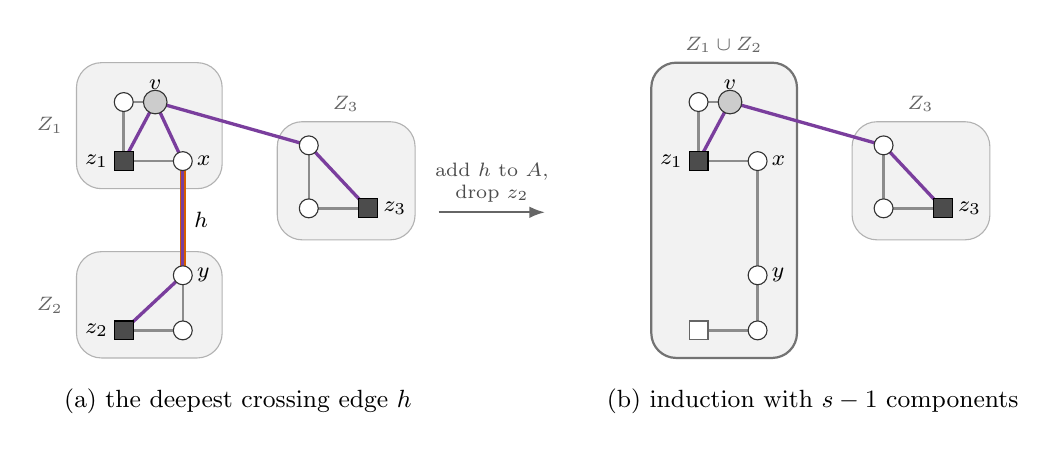
\begin{tikzpicture}[
  every node/.style={font=\footnotesize},
  v/.style={circle,draw=black!80,fill=white,inner sep=0pt,minimum size=2.4mm},
  sp/.style={rectangle,draw=black,fill=black!70,inner sep=0pt,minimum size=2.4mm},
  spoff/.style={rectangle,draw=black!60,fill=white,inner sep=0pt,minimum size=2.4mm},
  aE/.style={black!45,line width=.9pt},
  tE/.style={auxpurple,line width=1.2pt},
  hE/.style={witnessorange,line width=2.2pt},
  zc/.style={rounded corners=9pt,fill=black!5,draw=black!30},
  zm/.style={rounded corners=9pt,fill=black!5,draw=black!55,line width=.8pt},
  arr/.style={-{Latex[length=2mm]},line width=.8pt,black!60},
  lbl/.style={font=\scriptsize,text=black!60},
]
\newcommand{\staticbase}{%
  \coordinate (v) at (1.0,1.7); \coordinate (a1) at (0.6,1.7); \coordinate (z1) at (0.6,0.95);
  \coordinate (p) at (1.35,0.95);
  \coordinate (y) at (1.35,-0.5); \coordinate (a2) at (1.35,-1.2); \coordinate (z2) at (0.6,-1.2);
  \coordinate (q) at (2.95,1.15); \coordinate (a3) at (2.95,0.35); \coordinate (z3) at (3.7,0.35);}
\newcommand{\staticlabels}{%
  \node[anchor=south,inner sep=4.5pt] at (v) {$v$};
  \node[anchor=west,inner sep=5pt] at (p) {$x$};
  \node[anchor=west,inner sep=5pt] at (y) {$y$};}
% ================= panel (a) =================
\begin{scope}
  \staticbase
  \draw[zc] (0,0.6) rectangle (1.85,2.2);  \node[lbl,anchor=east] at (-0.05,1.4) {$Z_1$};
  \draw[zc] (0,-1.55) rectangle (1.85,-0.2); \node[lbl,anchor=east] at (-0.05,-0.88) {$Z_2$};
  \draw[zc] (2.55,-0.05) rectangle (4.3,1.45); \node[lbl,anchor=south] at (3.42,1.45) {$Z_3$};
  \draw[aE] (v)--(a1)--(z1)--(p) (y)--(a2)--(z2) (q)--(a3)--(z3);
  \draw[tE] (v)--(z1) (v)--(p) (y)--(z2) (v)--(q)--(z3);
  \draw[hE] (p)--(y);
  \draw[tE] (p)--(y);
  \node[anchor=west,inner sep=4pt] at (1.35,0.2) {$h$};
  \foreach \u in {p,y,a1,a2,a3,q} \node[v] at (\u) {};
  \node[v,fill=black!20,minimum size=3mm] at (v) {};
  \foreach \u in {z1,z2,z3} \node[sp] at (\u) {};
  \node[anchor=east,inner sep=5.5pt] at (z1) {$z_1$};
  \node[anchor=east,inner sep=5.5pt] at (z2) {$z_2$};
  \node[anchor=west,inner sep=5.5pt] at (z3) {$z_3$};
  \staticlabels
  \node[panel] at (2.05,-2.1) {(a) the deepest crossing edge $h$};
\end{scope}
\draw[arr] (4.6,0.3)--node[above,font=\scriptsize,text=black!70,align=center]{add $h$ to $A$,\\drop $z_2$}(5.95,0.3);
% ================= panel (b) =================
\begin{scope}[xshift=7.3cm]
  \staticbase
  \draw[zm] (0,-1.55) rectangle (1.85,2.2); \node[lbl,anchor=south] at (0.92,2.2) {$Z_1\cup Z_2$};
  \draw[zc] (2.55,-0.05) rectangle (4.3,1.45); \node[lbl,anchor=south] at (3.42,1.45) {$Z_3$};
  \draw[aE] (v)--(a1)--(z1)--(p) (y)--(a2)--(z2) (q)--(a3)--(z3) (p)--(y);
  \draw[tE] (v)--(z1) (v)--(q)--(z3);
  \foreach \u in {p,y,a1,a2,a3,q} \node[v] at (\u) {};
  \node[v,fill=black!20,minimum size=3mm] at (v) {};
  \foreach \u in {z1,z3} \node[sp] at (\u) {};
  \node[spoff] at (z2) {};
  \node[anchor=east,inner sep=5.5pt] at (z1) {$z_1$};
  \node[anchor=west,inner sep=5.5pt] at (z3) {$z_3$};
  \staticlabels
  \node[panel] at (2.05,-2.1) {(b) induction with $s-1$ components};
\end{scope}
\end{tikzpicture}
\caption{The induction step of \Cref{lem:characterization-static-selection}.
Gray edges belong to $A$ and form the components $Z_i$, each with a
specified vertex $z_i$ (squares); purple edges form a minimal tree
$T$ with $E(T)\subseteq D$ containing $v$ and all $z_i$, rooted at $v$. (a) The
crossing edge $h=xy$ of $T$ with $x$ deepest has its whole subtree below
$y$ inside one component, here $Z_2$, and only the $v$-$z_2$ path uses it.
(b) Adding $h$ to $A$ merges $Z_2$ with the component of $x$, and $z_2$ is
no longer specified. The path selected by induction avoids $h$ and is
also nonseparating in the original graph.}
\label{fig:static-selection}
\end{figure}

\begin{lemma}\label{lem:characterization-static-selection}
Let $J$ be a graph with disjoint edge sets $A,D$. The graph
$(V(J),A)$ has components $Z_1,\ldots,Z_s$, and each $Z_i$ contains
a specified vertex $z_i$. Suppose $D$ connects a vertex $v$ to every
$z_i$. Then some $v$-$z_i$ path in $D$ can be deleted from $J$
while leaving $J$ connected.
\end{lemma}
\begin{proof}
We induct on $s$. It suffices to retain $A$ and a minimal tree $T$
containing $v,z_1,\ldots,z_s$, with $E(T)\subseteq D$.
If $v$ is one of the specified vertices, choose
the trivial path. If $s=1$, deleting any $v$-$z_1$ path of $T$
leaves the connected spanning graph $(V(J),A)$.

For $s\ge2$, root $T$ at $v$. Choose an edge $h=xy$ joining
distinct components of $(V(J),A)$, with $x$ the parent of $y$ and
$x$ as deep as possible. Such an edge exists because $T$ connects
specified vertices in different components. By the choice of $h$,
all vertices in the subtree rooted at $y$ lie in the same component
$Z_i$. Minimality of $T$ ensures that this subtree contains a specified
vertex, which must be $z_i$. Thus $h$ is used by the $v$-$z_i$ path
and by none of the other specified root paths. Let $Z_j$ be the
component containing $x$, where $j\ne i$. Add $h$ to $A$, merging
$Z_i,Z_j$.
Discard $z_i$ from the specified list and let $D'$ be the union of
the edge sets of the remaining root paths, keeping the full vertex set and
$A\cup\{h\}$. The merged component retains $z_j$, and every other
component retains its specified vertex. The remaining root paths
avoid $h$, so induction applies with $s-1$ components and the
disjoint connecting edge set $D'$. Its selected path also leaves the original
graph $J$ connected when deleted.
\end{proof}

In the ordered setting, gathering paths reach the endpoints of
external calls before those calls occur, and connecting paths leave
those endpoints afterward. Restricting to maximal external calls
makes the two collections of internal edges disjoint. Paths between
comparable external calls ensure that the retained endpoints still
suffice for gathering, allowing us to apply the preceding lemma.

\begin{lemma}\label{lem:characterization-antichain-selection}
Let $J$ be a subgraph of a graph whose calls carry a partial order
$P$. Let $t_1,\ldots,t_k$ be external calls with endpoints $z_i$ in
$J$, and fix $v\in V(J)$. All comparisons and increasing paths below
use the restriction of $P$ to $E(J)\cup\{t_1,\ldots,t_k\}$. Suppose:
\begin{enumerate}
\item every vertex of $J$ has an internal increasing path to some
 $z_i$, all of whose calls precede $t_i$;
\item every $z_i$ has an internal increasing path to $v$, all of
 whose calls follow $t_i$;
\item if $t_i<t_j$, there is an internal increasing path from $z_i$
 to $z_j$ whose calls lie strictly between $t_i$ and $t_j$.
\end{enumerate}
Then some $z_i$-$v$ path can be deleted while retaining connectivity
of $J$. The selected path uses only calls from the paths in (2).
\end{lemma}
\begin{proof}
Retain only maximal calls among $t_1,\ldots,t_k$. Condition (3)
extends every gathering path in (1) to the port of a maximal call,
so these ports still suffice. Let $A$ be the union of the edge sets of
their gathering paths and $D$ the union of the edge sets of their
paths in (2). These edge sets are
disjoint: a common call would satisfy $t_i<a<t_j$ for two maximal
calls, a contradiction. Every component of $(V(J),A)$ contains a
port. Choose one port in each component and apply
\Cref{lem:characterization-static-selection}.
\end{proof}

The next lemma completes the quotient forest construction once a
compatible four-cycle has been selected. It does not select the
original attachment paths.

\begin{lemma}\label{lem:characterization-protected-extension}
Suppose $Q$ contains no nontrivial two-tree set, has $2r-4$ edges,
and has the canonical partition $I,F$ of
\Cref{lem:characterization-canonical-ideal}. Let $Y$ be its other early tree.
Suppose $g=u_0u_1$ is an edge of $Y$ and
$f_i=x_iu_i\in F$ for $i=0,1$. Then the four-cycle with edges
$e,g,f_0,f_1$ extends to an $M$-witness of $Q$ whose two forests
each have exactly one of $x_0,x_1,u_0,u_1$ in every component.
\end{lemma}
\begin{proof}
Start with the spanning tree $B=Q[F]+e$. Its complement
$K=Q[I\setminus\{e\}]$
has three distinguished tree components: the two parts $A_0,A_1$
of $X-e$ and the tree $Y$. Every other component is unicyclic by
\Cref{cor:characterization-early-components}. Among spanning trees $B$
containing $e,f_0,f_1$ but not $g$, whose complements have three
distinct tree components containing $x_0,x_1,u_0$ and all other
components unicyclic, minimize the number of complementary components.
The initial tree $Q[F]+e$ satisfies these conditions. Write
$K=Q-E(B)$ for the complement of the chosen tree. Since $g=u_0u_1$
remains in the complement, $u_1$ belongs to the component of $u_0$.

For a remaining unicyclic component $Z$, every edge of $K[V(Z)]$
joining different components of $B[V(Z)]$ is a bridge of $K[V(Z)]$.
Otherwise add such a nonbridge edge $h$ to $B$ and remove a tree
edge $t$ on its fundamental cycle crossing the boundary of $Z$.
The edge $t$ is none of $e,f_0,f_1$: all their endpoints lie in the
three distinguished components, whereas $t$ crosses the boundary of
$Z$. The edge $g$ remains in the complement. The new complement consists of $Z-h$ joined to
another component by $t$. If that component is a tree, the merge
is a tree; if it is unicyclic, the merge is unicyclic. None of the
distinguished components merge with each other. Thus the three specified
vertices remain in distinct tree components, and all other components
remain unicyclic. This reduces the component count, a
contradiction.

Since $Z$ is unicyclic, the bridge property puts its unique cycle
inside the vertex set $W$ of one component of $B[V(Z)]$.
The set $W$ is a proper subset of $V(Z)$: otherwise
$B[V(Z)]$ and a spanning tree of $K[V(Z)]$ would be two edge-disjoint spanning
trees on $V(Z)$. Replace the tree $B[W]$ using
\Cref{lem:characterization-exchange} on $Q[W]$. The new internal complement
is a forest whose partition coarsens the old one. If the old internal
complement has $q$ components, it has $|W|-q+1$ edges, since exactly
one component contains the unique cycle of $Z$. The new complement has
the same number of edges and is a forest, so it has $q-1$ components.
Since its partition coarsens the old one, two old internal complementary
components merge.

Globally the complementary vertex components remain unchanged, and
the component $Z$ stays connected. Its number of edges is unchanged,
so it remains unicyclic. The vertex components of $B[V(Z)]$ also remain
unchanged. Since $W\subseteq V(Z)$, the edges $e,f_0,f_1,g$ are untouched,
and the new tree satisfies the same minimizing conditions.
But an old complementary path
between the newly merged pieces leaves $W$ and crosses an unchanged
bridge joining distinct components of $B[V(Z)]$. The new internal
connections preserve every old internal complementary component
without using the bridge, since the bridge leaves $W$. Thus the
old connections on either side of its cut remain, and the newly
joined pieces connect the sides without the bridge. This makes
that bridge a nonbridge, contradicting the bridge
property for the equally minimizing new tree. Thus no unicyclic
component remains.

The resulting complement $K'=Q-E(B)$ is a forest with $r-3$ edges and three
components containing $x_0,x_1,u_0$ separately. Set
\[
 L_1=K'-g,\qquad L_2=B-\{e,f_0,f_1\}.
\]
Since $g$ lies in the tree component containing $u_0,u_1$, deleting it
separates these two vertices. The first forest therefore has four
components separating the four specified vertices.
The second does too, because its three removed edges form the path
$u_0,x_0,x_1,u_1$ in a spanning tree. Both avoid the four-cycle,
and they are edge-disjoint from each other. Each of their components
contains exactly one cycle vertex.
\end{proof}

\begin{figure}[t]
\centering
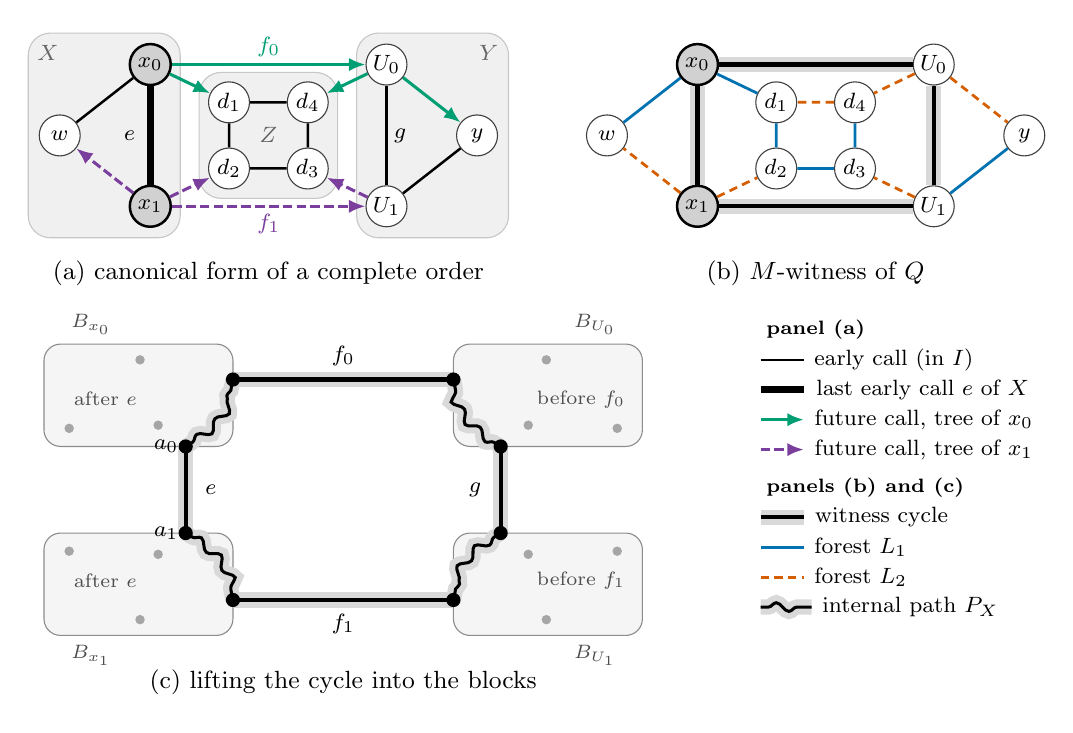
\begin{tikzpicture}[every node/.style={font=\footnotesize},
  early/.style={black,line width=.9pt},
  lastcall/.style={black,line width=2.4pt},
  fut0/.style={auxgreen,line width=1.1pt,-{Latex[length=2.1mm,width=1.7mm]}},
  fut1/.style={auxpurple,line width=1.1pt,dash pattern=on 3.5pt off 1.5pt,
               -{Latex[length=2.1mm,width=1.7mm]}},
  comp/.style={rounded corners=8pt,fill=black!6,draw=black!22},
  witcycle/.style={black,line width=1.5pt,preaction={draw,black!15,line width=5.5pt}},
  blk/.style={rounded corners=6pt,draw=black!45,fill=black!4},
  port/.style={circle,fill=black,inner sep=0pt,minimum size=1.8mm},
  inner/.style={circle,fill=black!35,inner sep=0pt,minimum size=1.2mm},
  ipath/.style={line width=1.1pt,decorate,decoration={snake,amplitude=.55mm,
               segment length=3.2mm,pre length=1mm,post length=1mm},
               preaction={draw,black!15,line width=5.5pt}},
  calledge/.style={witcycle},
  note/.style={font=\scriptsize,text=black!70}]
% Common vertex positions of the quotient Q in panels (a) and (b).
\def\placeQ{%
  \node[root] (x0) at (0,0.9) {$x_0$};
  \node[root] (x1) at (0,-0.9) {$x_1$};
  \node[vertex] (w) at (-1.15,0) {$w$};
  \node[vertex] (U0) at (3,0.9) {$U_0$};
  \node[vertex] (U1) at (3,-0.9) {$U_1$};
  \node[vertex] (y) at (4.15,0) {$y$};
  \node[vertex] (d1) at (1,0.42) {$d_1$};
  \node[vertex] (d2) at (1,-0.42) {$d_2$};
  \node[vertex] (d3) at (2,-0.42) {$d_3$};
  \node[vertex] (d4) at (2,0.42) {$d_4$};}
% ---------------- panel (a): canonical form ----------------
\begin{scope}
  \fill[comp] (-1.55,-1.3) rectangle (0.38,1.3);
  \fill[comp] (0.62,-0.8) rectangle (2.38,0.8);
  \fill[comp] (2.62,-1.3) rectangle (4.55,1.3);
  \node[text=black!60] at (-1.3,1.05) {$X$};
  \node[text=black!60] at (4.3,1.05) {$Y$};
  \node[text=black!60] at (1.5,0) {$Z$};
  \placeQ
  % early calls (the ideal I); e is the unique maximal call of X
  \draw[early] (w)--(x0) (y)--(U1) (d1)--(d2)--(d3)--(d4)--(d1);
  \draw[early] (U0)--(U1) node[midway,right=-1pt] {$g$};
  \draw[lastcall] (x0)--(x1) node[midway,left=1pt] {$e$};
  % future calls F, directed away from the roots
  \draw[fut0] (x0)--(U0) node[midway,above=-1pt] {$f_0$};
  \draw[fut0] (x0)--(d1);
  \draw[fut0] (U0)--(d4);
  \draw[fut0] (U0)--(y);
  \draw[fut1] (x1)--(U1) node[midway,below=-1pt] {$f_1$};
  \draw[fut1] (x1)--(d2);
  \draw[fut1] (U1)--(d3);
  \draw[fut1] (x1)--(w);
  \node[panel] at (1.5,-1.75) {(a) canonical form of a complete order};
\end{scope}
% ---------------- panel (b): quotient M-witness ----------------
\begin{scope}[xshift=6.95cm]
  \placeQ
  \draw[witcycle] (x0)--(U0)--(U1)--(x1)--(x0);
  \draw[blueforest] (d1)--(d2)--(d3)--(d4) (w)--(x0) (y)--(U1) (x0)--(d1);
  \draw[orangeforest] (d4)--(d1) (x1)--(d2) (U0)--(d4) (U1)--(d3)
                      (x1)--(w) (U0)--(y);
  \node[panel] at (1.5,-1.75) {(b) $M$-witness of $Q$};
\end{scope}
% ---------------- panel (c): lifting into the blocks ----------------
\begin{scope}[yshift=-4.5cm,xshift=-0.15cm]
  % Each block: center (cx,cy); (hx,vy) points towards the cycle's inside.
  \foreach \cx/\cy/\hx/\vy/\nm/\nt in {0/1.2/1/-1/{$B_{x_0}$}/{after $e$},
      5.2/1.2/-1/-1/{$B_{U_0}$}/{before $f_0$},
      5.2/-1.2/-1/1/{$B_{U_1}$}/{before $f_1$},
      0/-1.2/1/1/{$B_{x_1}$}/{after $e$}}{
    \draw[blk] (\cx-1.2,\cy-0.65) rectangle (\cx+1.2,\cy+0.65);
    \node[note] at (\cx-\hx*0.6,\cy-\vy*0.9) {\nm};
    \node[note] at (\cx-\hx*0.42,\cy+\vy*0.05) {\nt};
    \foreach \dx/\dy in {-0.88/0.42,0.02/-0.45,0.25/0.38}
      \node[inner] at (\cx+\hx*\dx,\cy+\vy*\dy) {};
    \coordinate (v) at (\cx+\hx*0.6,\cy+\vy*0.65);
    \coordinate (h) at (\cx+\hx*1.2,\cy-\vy*0.2);
    \pgfmathsetmacro{\bend}{-25*\hx*\vy}
    \draw[ipath] (v) to[bend right=\bend] (h);
  }
  % lifted external calls between the ports
  \draw[calledge] (0.6,0.55)--(0.6,-0.55) node[midway,right=3pt] {$e$};
  \draw[calledge] (1.2,1.4)--(4.0,1.4) node[midway,above=1pt] {$f_0$};
  \draw[calledge] (4.6,0.55)--(4.6,-0.55) node[midway,left=3pt] {$g$};
  \draw[calledge] (4.0,-1.4)--(1.2,-1.4) node[midway,below=1pt] {$f_1$};
  \foreach \p in {(0.6,0.55),(1.2,1.4),(4.0,1.4),(4.6,0.55),
                  (4.6,-0.55),(4.0,-1.4),(1.2,-1.4),(0.6,-0.55)}
    \node[port] at \p {};
  \node[anchor=east,inner sep=2.5pt] at (0.6,0.55) {$a_0$};
  \node[anchor=east,inner sep=2.5pt] at (0.6,-0.55) {$a_1$};
  \node[panel] at (2.6,-2.45) {(c) lifting the cycle into the blocks};
\end{scope}
% ---------------- legend ----------------
\begin{scope}[xshift=7.75cm,yshift=-2.85cm]
  \node[anchor=west,font=\scriptsize\bfseries] at (-0.05,0.38) {panel (a)};
  \draw[early] (0,0)--(0.55,0) node[right,text=black] {early call (in $I$)};
  \draw[lastcall] (0,-0.38)--(0.55,-0.38) node[right,text=black] {last early call $e$ of $X$};
  \draw[fut0] (0,-0.76)--(0.55,-0.76) node[right,text=black] {future call, tree of $x_0$};
  \draw[fut1] (0,-1.14)--(0.55,-1.14) node[right,text=black] {future call, tree of $x_1$};
  \node[anchor=west,font=\scriptsize\bfseries] at (-0.05,-1.62) {panels (b) and (c)};
  \draw[witcycle] (0,-2.0)--(0.55,-2.0) node[right,text=black] {witness cycle};
  \draw[blueforest] (0,-2.38)--(0.55,-2.38) node[right,text=black] {forest $L_1$};
  \draw[orangeforest] (0,-2.76)--(0.55,-2.76) node[right,text=black] {forest $L_2$};
  \draw[ipath] (0,-3.14)--(0.65,-3.14) node[right,text=black] {internal path $P_X$};
\end{scope}
\end{tikzpicture}
\caption{The necessity proof of \Cref{thm:characterization} on a quotient
$Q$ with $r=10$ vertices and $2r-4=16$ edges that contains no nontrivial
two-tree set. A complete call order is $d_1d_2$, $d_3d_4$, $d_2d_3$,
$d_4d_1$, $wx_0$, $yU_1$, $U_0U_1$, $x_0x_1$, followed by $x_0U_0$,
$x_1U_1$, $x_0d_1$, $x_1d_2$, $U_0d_4$, $U_1d_3$, $x_1w$, $U_0y$; every
linear extension of its causal order is complete.
(a) The canonical form of
\Cref{lem:characterization-canonical-ideal,cor:characterization-early-components}.
The early calls form the tree components $X$ and $Y$ and the unicyclic
component $Z$; the call $e=x_0x_1$ is the unique maximal call of $X$
and precedes every future call. The future calls form two trees rooted at
$x_0$ and $x_1$ and are ordered outward from the roots; the minimal
future calls $f_0,f_1$ join $X$ to $Y$. Here
$f_i=f_{U_i}=x_iU_i$ for $i\in\{0,1\}$.
(b) The $M$-witness of $Q$
obtained from the four-cycle $(x_0,U_0,U_1,x_1)$ by
\Cref{lem:characterization-protected-extension}: the exchange moves the
early call $d_4d_1$ into the spanning tree $Q[F]+e$ and the future call
$x_0d_1$ out of it, which removes the unicyclic component.
(c) Lifting to $G$ (\Cref{lem:characterization-m-lift}), shown
schematically. Each quotient vertex represents an original block.
To lift the witness, each block on the cycle needs two spanning trees
and a path between its two ports---the original endpoints of its
incident cycle edges---with all three edge sets pairwise disjoint.
In $B_{x_i}$, the path uses calls after $e$, and deleting it leaves
those calls connected, providing one spanning tree; the calls before
$e$ provide the other. In $B_{U_i}$, the path and the first spanning
tree use calls before $f_i$, while the second spanning tree uses
calls after $f_i$
(\Cref{lem:characterization-threshold,lem:characterization-compatible-actual-cycle}).}
\label{fig:necessity-canonical}
\end{figure}

\subsection{Selecting Compatible Ports Using Original Routes}
\label{sec:necessity-ports}

We now carry out the final stage of the necessity proof: select a
four-cycle in the quotient whose witness can be lifted to the original
graph. Finding the cycle alone is not enough. In each original block
on the cycle, its two attachment vertices---called \emph{ports}---must
be joined by a path such that this path and two spanning trees of the
block are pairwise edge-disjoint. We use information routes in the
original graph to select the quotient edges and guarantee these
internal paths. We then extend the four-cycle to an $M$-witness using
\Cref{lem:characterization-protected-extension} and lift that witness
using \Cref{lem:characterization-m-lift}.

We keep the original causal order $P$ and its restriction $P_Q$ to
external calls. Throughout this section, $Q$ has $r\ge4$ vertices and
$2r-4$ edges, and $I,F,X,Y,e=x_0x_1$ are as in
\Cref{lem:characterization-canonical-ideal} and
\Cref{cor:characterization-early-components}. Let $B_U$ denote the original
block represented by a quotient vertex $U$. For an external call $a$
incident with $U$, write $p_U(a)$ for its original endpoint in $B_U$.
In particular, let $a_i=p_{x_i}(e)$ for $i\in\{0,1\}$.

An \emph{original route} is a path in $G$ whose successive calls
increase in $P$. Completeness supplies such a route between every
ordered pair of original vertices. Its external projection is a
$P_Q$-increasing trail: its edges are distinct, although its quotient
vertices may repeat. For an original block $B$ and a call $t$, define
\[
 J_B^-(t)=\bigl(B,\{a\in E(G[B]):a<_P t\}\bigr),\qquad
 J_B^+(t)=\bigl(B,\{a\in E(G[B]):t<_P a\}\bigr).
\]
These graphs retain every vertex of $B$. In the following, calls before
or after $t$ mean predecessors or successors of $t$ in the causal
order $P$. All paths below may be
trivial. Deleting the edges of a trivial path leaves the graph
unchanged.

The selection has three steps. First, retain routes whose final
attachment to $B_{x_i}$ admits an internal path whose deletion
preserves the required connectivity. Second, use these routes to find
a connected set of blocks in which internal return paths can be
forced. Third, select two adjacent blocks with routes to different
roots and compatible ports at both ends. We begin with the confinement and connectivity facts
needed in the first two steps.

\begin{lemma}[Confinement to a quotient forest]
\label{lem:characterization-forest-confinement}
Let $a<_{P_Q}b$ be external calls sharing a quotient vertex $U$.
Suppose a quotient forest $R$ contains $a,b$ and every external call
$c$ with $a<_{P_Q}c<_{P_Q}b$. Then there is an internal original
route from $p_U(a)$ to $p_U(b)$ whose calls lie strictly between
$a$ and $b$ in $P$.
\end{lemma}
\begin{proof}
Place a marker at both endpoints immediately after call $a$.
A causal chain from $a$ to $b$ implies that at least one endpoint of
$b$ receives the marker before $b$. Use only the intermediate calls
of this chain to transmit the marker. Tracing these transmissions gives
an increasing original path, using calls strictly between $a,b$ in $P$,
from an endpoint of $a$ to an endpoint of $b$.

Every external call of this path belongs to $R-\{a,b\}$. Deleting
$a,b$ from the forest separates their two nonshared endpoints from
each other and from their common endpoint $U$. Thus the only possible
match between an endpoint component of $a$ and an endpoint component
of $b$ is the component containing $U$. The path therefore starts at
$p_U(a)$ and ends at $p_U(b)$. Its external projection is a closed
trail from $U$ to $U$ in a forest, so it is empty. The path is internal
to $B_U$.
\end{proof}

We will apply this lemma in three settings. Comparisons between early
calls in the same early tree are confined to that tree. Indeed, $I$
is an ideal, and a causal chain between its external calls cannot
leave an early component: consecutive external calls of a causal
chain share a quotient vertex. Comparisons between future calls are
confined to $F$, since $I$ is an ideal. Finally, comparisons from $e$
to future calls are confined to the tree $Q[F]+e$. To see this, $e$ is
maximal in $I$: a chain of incident early calls cannot leave $X$,
and $e$ is maximal in $X$. Hence no other early call lies above $e$.

\begin{lemma}[Internal connectivity at the relevant thresholds]
\label{lem:characterization-internal-threshold-connectivity}
For each $i\in\{0,1\}$, the graphs
$J_{B_{x_i}}^-(e)$ and $J_{B_{x_i}}^+(e)$ are connected.
Moreover, if $U\in V(Y)$ and $f=Ux_i\in F$, then $J_{B_U}^+(f)$
is connected.
\end{lemma}
\begin{proof}
Fix an original vertex $z\in B_{x_i}$ and an original route from
$z$ to $a_{1-i}$. Its first external call lies in $I$. Otherwise
all its external calls would lie in $F$, and a trail in $F$ could
not connect its different root components. Denote this first call
by $a$. The call $a$ belongs to $X$ and is incident with $x_i$.
If $a=e$, the initial internal segment gathers $z$ to $a_i$ before
$e$. Otherwise $a<_{P_Q}e$, and
\Cref{lem:characterization-forest-confinement}, applied in $X$, gives an internal
route from $p_{x_i}(a)$ to $a_i$ between $a,e$. Concatenate it with
the initial internal segment. Erasing closed subwalks gives an
internal route from $z$ to $a_i$ before $e$. These routes prove that
$J_{B_{x_i}}^-(e)$ is connected.

Next take an original route from $a_{1-i}$ to $z$.
\Cref{lem:characterization-canonical-ideal} applies to its external trail ending
at $x_i$. Its last external call is either $e$ or a future call $t$
incident with $x_i$. Indeed, if there were no future call, the unique
early-tree path from $x_{1-i}$ to $x_i$ would use $e$.
If the last call is $e$, its internal suffix starts at $a_i$ and
lies after $e$. Otherwise $e<_{P_Q}t$, and confinement in $Q[F]+e$
gives an internal route from $a_i$ to $p_{x_i}(t)$ between $e,t$.
Append the internal suffix following $t$. This proves that
$J_{B_{x_i}}^+(e)$ is connected.

Finally, fix $U\in V(Y)$ with $f=Ux_i\in F$ and an original
vertex $z\in B_U$. Take an original route from $a_i$ to $z$.
Some external call of this route lies in $F$, since its endpoints
belong to different early components. All external calls after the
first future call remain in $F$. Let $t$ be its last external call,
which is incident with $U$. If $t=f$, its internal suffix gathers
$p_U(f)$ to $z$ after $f$. Otherwise $t$ is an edge from $U$ to one
of its future children. The outward order gives $f<_{P_Q}t$.
Confinement in $F$ gives an internal route from $p_U(f)$ to $p_U(t)$
between $f,t$; append the suffix following $t$. Thus every original
vertex of $B_U$ is internally reachable from $p_U(f)$ after $f$.
\end{proof}

\subsubsection{Filtering Routes}

We first ensure that each root block $B_{x_i}$, for $i\in\{0,1\}$,
contains two spanning trees and a path between its two cycle ports,
with all three edge sets pairwise disjoint, as required by
\Cref{lem:characterization-m-lift}. A route entering $B_{x_i}$ through
a future call $t$ determines the port $p_{x_i}(t)$. We retain only
routes for which this port can be joined to the port $a_i$ of $e$ by
a path in $J_{B_{x_i}}^+(e)$ whose deletion leaves that graph connected.
The remaining edges of this graph supply one spanning tree, and
$J_{B_{x_i}}^-(e)$ supplies the other. We show that every original source in a
block represented in $Y$ still has a retained route to each root block.

For $i\in\{0,1\}$, call a future edge $t=Vx_i$ with $V\in V(Y)$
\emph{good at $x_i$} if there is an $a_i$-$p_{x_i}(t)$ path in $J_{B_{x_i}}^+(e)$ whose
deletion leaves $J_{B_{x_i}}^+(e)$ connected. This property concerns
only the edge $t$ and its endpoint $p_{x_i}(t)$ in $B_{x_i}$.

\begin{lemma}\label{lem:characterization-root-good-routes}
For every original vertex $u$ in a block represented in $Y$ and each
$i\in\{0,1\}$, there is an original route from $u$ to some original
vertex of $B_{x_i}$ whose last external call is good at $x_i$.
\end{lemma}
\begin{proof}
For every original vertex $v\in B_{x_i}$, choose an original
$u$-$v$ route. Its external projection ends at $x_i$.
The last assertion of \Cref{lem:characterization-canonical-ideal} implies that
this projection is an early path in $Y$ followed by a single future
edge $t_v=V_vx_i$. In particular, it cannot use $e$: an early prefix
starting in $Y$ cannot reach $X$.

The internal suffix from $p_{x_i}(t_v)$ to $v$ lies after $t_v$.
Confinement in $Q[F]+e$ gives an internal route from $a_i$ to
$p_{x_i}(t_v)$ between $e,t_v$. Whenever two selected future calls
are comparable, confinement in $F$ gives an internal route between
their ports strictly between those calls.

Apply \Cref{lem:characterization-antichain-selection} with the call order reversed to the
internal graph $J_{B_{x_i}}^+(e)$, with distinguished vertex $a_i$
and external calls $t_v$. The reversed suffixes supply its gathering
paths, the reversed routes from $a_i$ to $p_{x_i}(t_v)$ supply its connecting paths,
and the confined between-call routes supply its third condition.
Repeated calls $t_v$ are identified; all occurrences have the same
endpoint in $B_{x_i}$, and their suffixes still cover all targets.
Every used internal call lies after $e$. The lemma selects one
$t_v$ good at $x_i$, and the associated chosen original route proves
the assertion. Its target may be any vertex of $B_{x_i}$; no claim
that it ends specifically at $a_i$ is needed.
\end{proof}

A \emph{filtered route with root index $i$} starts at an original vertex of
a block in $Y$, ends at any original vertex of $B_{x_i}$, and has a
last external call good at $x_i$. Every such route projects to an
early path in $Y$ followed by that last future call. For $U\in V(Y)$,
let $N_i(U)$ be the set of all vertices $V$ that occur immediately
before $x_i$ in these projections, ranging over \emph{all} filtered
routes starting at \emph{every} original vertex of $B_U$.
A nonempty set $S\subseteq V(Y)$ is \emph{closed} if
\[
 N_0(U)\cup N_1(U)\subseteq S\qquad\text{for every }U\in S.
\]
Thus every filtered route starting in a block represented in $S$
makes its final departure toward a root from a block still
represented in $S$.
The whole set $V(Y)$ is closed and induces a connected graph. Choose
$S$ inclusion-minimal among nonempty closed sets for which $Y[S]$ is
connected. \Cref{fig:filtered-routes} illustrates filtered routes and
closed sets, together with the internal return paths obtained from
the minimality of $S$.

\subsubsection{Obtaining Internal Return Paths}

Filtering provides suitable attachment paths inside the root blocks.
We now prepare the corresponding paths inside blocks represented by
the other early tree $Y$. Recall that $S$ is an inclusion-minimal
nonempty closed set for which $Y[S]$ is connected. We show that each
block represented in $S$ has a future call to a root and that every
incident edge of $Y[S]$ can be followed by an internal route to the
port of this future call. These routes will supply the connecting
paths needed by the ordered path-selection lemma,
\Cref{lem:characterization-antichain-selection}.

\begin{figure}[t]
\centering
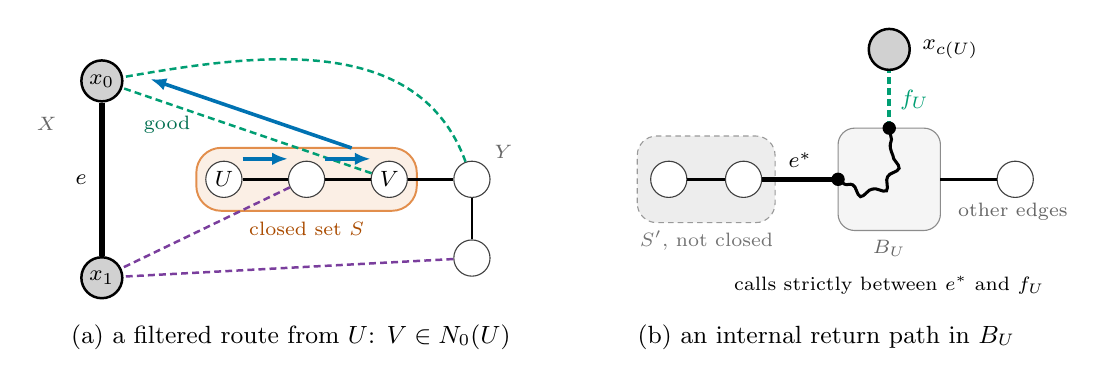
\begin{tikzpicture}[
  every node/.style={font=\footnotesize},
  qv/.style={circle,draw=black!75,fill=white,inner sep=0pt,minimum size=4.6mm},
  rootv/.style={circle,draw=black,fill=black!18,line width=.9pt,inner sep=0pt,minimum size=5.2mm},
  treeE/.style={black,line width=.9pt},
  lastE/.style={black,line width=2.4pt},
  fut0/.style={auxgreen,line width=.9pt,dash pattern=on 2.5pt off 1.5pt},
  fut1/.style={auxpurple,line width=.9pt,dash pattern=on 2.5pt off 1.5pt},
  route/.style={-{Latex[length=2mm,width=1.6mm]},line width=1.3pt,witnessblue},
  setS/.style={fill=witnessorange!10,draw=witnessorange!70,rounded corners=9pt,line width=.7pt},
  setSp/.style={fill=black!7,draw=black!40,rounded corners=7pt,dash pattern=on 2pt off 1.5pt},
  blk/.style={rounded corners=6pt,draw=black!45,fill=black!4},
  port/.style={circle,fill=black,inner sep=0pt,minimum size=1.7mm},
  ipath/.style={line width=1.1pt,decorate,decoration={snake,amplitude=.5mm,segment length=3mm,pre length=1mm,post length=1mm}},
  good/.style={font=\scriptsize,text=auxgreen!70!black},
]
% ================= panel (a) =================
\begin{scope}
  \node[rootv] (x0) at (0,1.25) {$x_0$};
  \node[rootv] (x1) at (0,-1.25) {$x_1$};
  \draw[lastE] (x0)--(x1) node[midway,left=1pt] {$e$};
  \node[font=\scriptsize,text=black!60] at (-0.7,0.7) {$X$};
  \draw[setS] (1.2,-0.4) rectangle (4.0,0.4);
  \node[qv] (y1) at (1.55,0) {$U$};
  \node[qv] (y2) at (2.6,0) {};
  \node[qv] (y3) at (3.65,0) {$V$};
  \node[qv] (y4) at (4.7,0) {};
  \node[qv] (y5) at (4.7,-1.0) {};
  \draw[treeE] (y1)--(y2)--(y3)--(y4)--(y5);
  \node[font=\scriptsize,text=black!60] at (5.1,0.35) {$Y$};
  \node[font=\scriptsize,text=witnessorange!80!black,anchor=north] at (2.6,-0.42) {closed set $S$};
  \draw[fut0] (y3)--(x0);
  \node[good] at ($(y3)!0.8!(x0)+(0.1,-0.3)$) {good};
  \draw[fut1] (y2)--(x1);
  \draw[fut1] (y5)--(x1);
  \draw[fut0] (y4) to[out=110,in=10] (x0);
  \draw[route] ([yshift=2.6mm]y1.east)--([yshift=2.6mm]y2.west);
  \draw[route] ([yshift=2.6mm]y2.east)--([yshift=2.6mm]y3.west);
  \draw[route] ($(y3)!0.15!(x0)+(0.07,0.21)$)--($(y3)!0.85!(x0)+(0.07,0.21)$);
  \node[panel,align=center] at (2.4,-2.0) {(a) a filtered route from $U$: $V\in N_0(U)$};
\end{scope}
% ================= panel (b) =================
\begin{scope}[xshift=7.4cm]
  \node[rootv] (r) at (2.6,1.65) {}; \node[anchor=west,inner sep=4pt] at (r.east) {$x_{c(U)}$};
  \draw[setSp] (-0.6,-0.55) rectangle (1.15,0.55);
  \node[font=\scriptsize,text=black!55] at (0.28,-0.78) {$S'$, not closed};
  \node[qv] (s1) at (-0.2,0) {};
  \node[qv] (s2) at (0.75,0) {};
  \draw[treeE] (s1)--(s2);
  \draw[blk] (1.95,-0.65) rectangle (3.25,0.65);
  \node[font=\scriptsize,text=black!60] at (2.6,-0.88) {$B_U$};
  \coordinate (pe) at (1.95,0); \coordinate (pf) at (2.6,0.65);
  \draw[treeE,line width=1.6pt] (s2)--(pe) node[midway,above] {$e^*$};
  \draw[fut0,line width=1.3pt] (pf)--(r) node[midway,right] {$f_U$};
  \draw[ipath] (pe) .. controls (2.35,-0.35) and (2.75,0.0) .. (pf);
  \node[qv] (s3) at (4.2,0) {};
  \draw[treeE] (3.25,0)--(s3);
  \node[font=\scriptsize,text=black!60,anchor=north west] at (3.35,-0.18) {other edges};
  \foreach \p in {pe,pf} \node[port] at (\p) {};
  \node[font=\scriptsize,anchor=north] at (2.6,-1.1) {calls strictly between $e^*$ and $f_U$};
  \node[panel,align=center] at (1.8,-2.0) {(b) an internal return path in $B_U$};
\end{scope}
\end{tikzpicture}
\caption{Filtered routes and minimal closed sets
(\Cref{lem:characterization-root-good-routes,lem:characterization-actual-closed-set}).
(a) A filtered route projects to an early path in $Y$ followed by one
future call to a root block, here from $V$ to $x_0$; its last call is good
at that root. The vertex $V$ is then in $N_0(U)$. A set $S$ of vertices of
$Y$ is closed if every filtered route starting in a block represented
in $S$ makes its final departure toward a root from a block represented
in $S$. (b) Let $S$ be inclusion-minimal among nonempty closed sets
inducing a connected subgraph of $Y$, and let $U\in S$. Let $e^*$ be a
maximal edge of $Y[S]$ at $U$. The vertex set $S'$ of the
component of $Y[S]-e^*$ not containing $U$ is not closed, so some filtered route
starting in $S'$ leaves it. That route crosses $e^*$ into the block $B_U$
and leaves it through the future call $f_U$ to a root. Its segment inside
$B_U$ (wavy) uses only calls between $e^*$ and $f_U$.}
\label{fig:filtered-routes}
\end{figure}

\begin{lemma}[Minimal closed sets supply internal returns]
\label{lem:characterization-actual-closed-set}
The graph $Y[S]$ is a tree with at least two vertices. Every $U\in S$
has a unique future edge $f_U=Ux_{c(U)}$ incident with a root, for a
root index $c(U)\in\{0,1\}$, and this edge is good at $x_{c(U)}$.
For every edge $h$ of $Y[S]$ incident with $U$, we have
$h<_{P_Q}f_U$, and there is an internal
original route from $p_U(h)$ to $p_U(f_U)$ with all calls strictly
between $h$ and $f_U$.
\end{lemma}
\begin{proof}
By its choice, $Y[S]$ is a connected subgraph of the tree $Y$, hence a tree.
A singleton closed set would require future edges from its sole
vertex to both roots, since every original source has a filtered
route of each root index by \Cref{lem:characterization-root-good-routes}. Those edges
would connect the two root components of $F$, which is impossible.
Consequently $|S|\ge2$.

Fix $U\in S$ and an edge $e^*$ maximal among the edges of $Y[S]$
incident with $U$. Let $S'$ be the vertex set of the component of
$Y[S]-e^*$ not containing $U$. Then $S'$ is a nonempty proper subset
of $S$, and $Y[S']$ is connected. By minimality of $S$, the set $S'$
is not closed. A witnessing filtered
route has its starting block in $S'$ and its exit in $S\setminus S'$.
It crosses $e^*$ into $U$ and cannot use another early edge, by
maximality of $e^*$. Its next external call is therefore a future edge
$f_U$ from $U$ to a root. This call is good at that root, and the
actual route gives $e^*<_{P_Q}f_U$, even if its internal segment is
trivial. That segment is the required return path.
There cannot be future edges from $U$ to both roots because the roots
lie in different components of $F$; simplicity gives uniqueness for
the chosen root. This proves the assertion for every maximal $e^*$.

For an arbitrary incident edge $h$, choose a maximal incident edge
$e^*$ with $h\le_{P_Q}e^*$. If $h\ne e^*$, confinement in the early tree
$Y$ supplies an internal original route from $p_U(h)$ to $p_U(e^*)$
between $h,e^*$. Append the return path just obtained between $e^*,f_U$.
In particular $h<_{P_Q}f_U$. The ordered call intervals give an
increasing internal walk; erase
closed subwalks. The resulting path lies strictly between $h,f_U$.
\end{proof}

\subsubsection{Selecting Neighbors with Different Root Indices}
Each vertex $U\in S$ now has a future edge $f_U$ to the root
$x_{c(U)}$. We seek adjacent vertices $U_0,U_1$ with different root
indices, so that their future edges, their common early edge, and
$e=x_0x_1$ form a four-cycle. At both ends of the common early edge,
we also need an internal path to the future port whose deletion
leaves the corresponding graph $J_{B_U}^-(f_U)$ connected. We first find
admissible neighbor choices at every vertex, then use a rerouting
argument to obtain a pair that chooses each other and has different
root indices.

\begin{lemma}\label{lem:characterization-safe-first-edges}
Fix $U\in S$. For every original vertex $u\in B_U$, choose a
filtered route with root index $1-c(U)$. Among their first external edges
there is an edge $h$ such that $J_{B_U}^-(f_U)$ contains a
$p_U(h)$-$p_U(f_U)$ path whose deletion leaves this graph connected.
\end{lemma}
\begin{proof}
The early projection of every chosen route stays in $Y[S]$ because
its starting block and its exit belong to $S$. Its first external
edge $h_u$ is early: the only root exit from $U$ has root index $c(U)$,
whereas the chosen route has the other root index. Its initial internal
segment gathers $u$ to $p_U(h_u)$ before $h_u$.
\Cref{lem:characterization-actual-closed-set} supplies an internal route from
$p_U(h_u)$ to $p_U(f_U)$ between $h_u,f_U$. All these gathering and
connecting paths lie in $J_{B_U}^-(f_U)$.

For any comparable chosen first edges $h_u<_{P_Q}h_v$, confinement
in $Y$ supplies the internal between-port route required by the
third condition of \Cref{lem:characterization-antichain-selection}. Its first
condition is supplied by the gathering prefixes, and its second by
the return paths to $p_U(f_U)$. That lemma gives the claimed edge
and nonseparating path. Repeated occurrences of the same first call
may be identified; they have the same original port.
\end{proof}

To find an early edge with compatible internal paths at both ends,
we encode the admissible choices at each block in a directed graph.

Define a directed graph $D$ on $S$, using only edges of $Y[S]$.
Include an arc $U\to V$ if there is a filtered route starting in
$B_U$ with root index $1-c(U)$ whose first external edge is $UV$, and
there is a
$p_U(UV)$-$p_U(f_U)$ path in $J_{B_U}^-(f_U)$ whose deletion
leaves that graph connected. The route and the nonseparating path
need not use the same internal edges.
\Cref{lem:characterization-safe-first-edges} shows that every vertex of $D$ has
positive outdegree. Its formulation also allows us to prescribe a
family of candidate routes before choosing the outgoing arc.

\begin{lemma}\label{lem:characterization-same-index-rerouting}
If $U\to V$ is an arc of $D$ and $c(U)=c(V)$, then $V$ has an
outgoing arc to a neighbor other than $U$.
\end{lemma}
\begin{proof}
Take a filtered route witnessing $U\to V$. Its terminal exit has
root index $1-c(U)$, so its early projection cannot end at $V$. Let $VW$
be its next external edge after $UV$. Between these calls the route
has an actual internal segment in $B_V$ from $p_V(UV)$ to $p_V(VW)$,
with all calls strictly between $UV,VW$.

For every original vertex $v\in B_V$, choose a filtered route with
root index $1-c(V)$. If its first external edge differs from $VU$, keep
it. Otherwise keep its internal prefix before $VU$, then append the
actual internal $V$-segment of the $U$-route and the suffix of that
route beginning with $VW$. The prefix ends at $p_V(VU)$ before
$VU$; the replacement segment starts at that same port after $UV$.
Hence this concatenation is an increasing original walk. Its first
external call is $VW$, and its last external call is still good at
the opposite root. The suffix after $VW$ never returns to $V$,
since its early projection is a path in $Y$. Erasing closed
subwalks inside $B_V$ therefore gives a filtered original route
whose first external edge differs from $VU$.

We have obtained such a candidate route for every original vertex
of $B_V$. Apply \Cref{lem:characterization-safe-first-edges} to these candidates.
The resulting outgoing arc of $V$ avoids $U$.
\end{proof}

\Cref{fig:port-selection} illustrates this rerouting step and the
selection of adjacent blocks with different root indices in the next
lemma.

\begin{figure}[t]
\centering
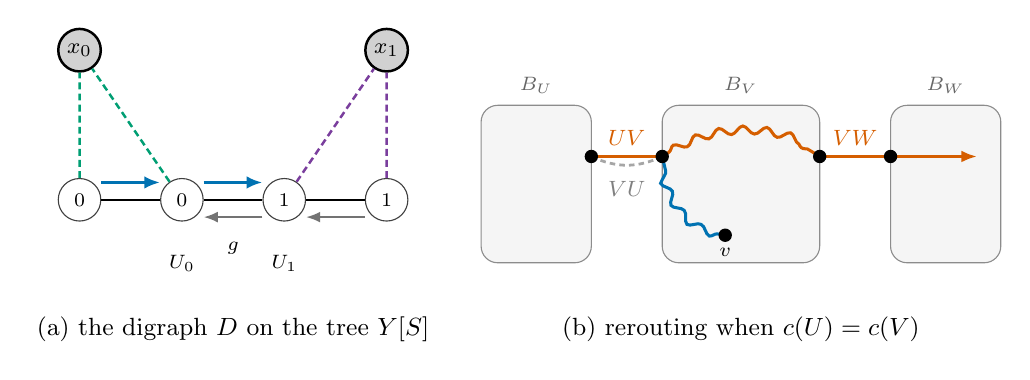
\begin{tikzpicture}[
    every node/.style={font=\footnotesize},
    qv/.style={circle,draw=black!75,fill=white,inner sep=0pt,minimum size=5.4mm},
    rootv/.style={circle,draw=black,fill=black!18,line width=.9pt,inner sep=0pt,minimum size=5.4mm},
    treeE/.style={black,line width=.9pt},
    fut0/.style={auxgreen,line width=.9pt,dash pattern=on 2.5pt off 1.5pt},
    fut1/.style={auxpurple,line width=.9pt,dash pattern=on 2.5pt off 1.5pt},
    arc/.style={-{Latex[length=1.8mm,width=1.4mm]},line width=.8pt,black!55},
    patharc/.style={-{Latex[length=2mm,width=1.6mm]},line width=1.3pt,witnessblue},
    gE/.style={black,line width=2.4pt},
    blk/.style={rounded corners=6pt,draw=black!45,fill=black!4},
    port/.style={circle,fill=black,inner sep=0pt,minimum size=1.7mm},
    ipath/.style={line width=1.1pt,decorate,decoration={snake,amplitude=.5mm,segment length=3mm,pre length=1mm,post length=1mm}},
    panel/.style={font=\small}
]
% ---------------- panel (a): the digraph D on Y[S] ----------------
\begin{scope}
  \node[rootv] (x0) at (0.0,1.9) {$x_0$};
  \node[rootv] (x1) at (3.9,1.9) {$x_1$};
  \node[qv] (A) at (0,0) {};
  \node[qv] (B) at (1.3,0) {};
  \node[qv] (C) at (2.6,0) {};
  \node[qv] (E) at (3.9,0) {};
  \draw[treeE] (A)--(B)--(C)--(E);
  \draw[fut0] (A)--(x0) (B)--(x0);
  \draw[fut1] (C)--(x1) (E)--(x1);
  \foreach \v/\c in {A/0,B/0,C/1,E/1} \node[font=\scriptsize] at (\v.center) {$\c$};
  % arcs of D, drawn beside the tree edges
  \draw[patharc] ([yshift=2.2mm]A.east)--([yshift=2.2mm]B.west);
  \draw[patharc] ([yshift=2.2mm]B.east)--([yshift=2.2mm]C.west);
  \draw[arc] ([yshift=-2.2mm]C.west)--([yshift=-2.2mm]B.east);
  \draw[arc] ([yshift=-2.2mm]E.west)--([yshift=-2.2mm]C.east);
  \node[font=\scriptsize] at (B.south) [below=3mm] {$U_0$};
  \node[font=\scriptsize] at (C.south) [below=3mm] {$U_1$};
  \node[font=\scriptsize] at (1.95,-0.62) {$g$};
  \node[panel,align=center] at (1.95,-1.65) {(a) the digraph $D$ on the tree $Y[S]$};
\end{scope}
% ---------------- panel (b): rerouting ----------------
\begin{scope}[xshift=6.0cm,yshift=0.2cm]
  \draw[blk] (-0.9,-1.0) rectangle (0.5,1.0);  \node[font=\scriptsize,text=black!60] at (-0.2,1.25) {$B_U$};
  \draw[blk] (1.4,-1.0) rectangle (3.4,1.0);   \node[font=\scriptsize,text=black!60] at (2.4,1.25) {$B_V$};
  \draw[blk] (4.3,-1.0) rectangle (5.7,1.0);   \node[font=\scriptsize,text=black!60] at (5.0,1.25) {$B_W$};
  \coordinate (pu) at (0.5,0.35); \coordinate (pv) at (1.4,0.35);
  \coordinate (qv) at (3.4,0.35); \coordinate (qw) at (4.3,0.35);
  \coordinate (v) at (2.2,-0.65);
  % U-route: UV, internal segment in B_V, VW
  \draw[witnessorange,line width=1.4pt] (pu)--(pv) node[midway,above] {$UV$};
  \draw[witnessorange,ipath] (pv) .. controls (2.0,0.75) and (2.8,0.75) .. (qv);
  \draw[witnessorange,line width=1.4pt] (qv)--(qw) node[midway,above] {$VW$};
  \draw[witnessorange,line width=1.4pt,-{Latex[length=2mm]}] (qw)--(5.4,0.35);
  % v-route prefix to the port of VU
  \draw[witnessblue,ipath] (v) .. controls (1.7,-0.6) and (1.5,-0.1) .. (pv);
  % its original exit via VU, discarded
  \draw[black!35,line width=1pt,dash pattern=on 2pt off 1.5pt] (pv) to[bend left=25] node[midway,below=2pt,text=black!50] {$VU$} (pu);
  \foreach \p in {pu,pv,qv,qw} \node[port] at (\p) {};
  \node[port] at (v) {}; \node[below=1pt,font=\scriptsize] at (v) {$v$};
  \node[panel,align=center] at (2.4,-1.85) {(b) rerouting when $c(U)=c(V)$};
\end{scope}
\end{tikzpicture}
\caption{Selecting adjacent blocks with different root indices
(\Cref{lem:characterization-same-index-rerouting,lem:characterization-compatible-actual-cycle}).
(a) The vertices of the tree $Y[S]$ carry their root indices $c(U)$,
and dashed edges show the future edges $f_U$ to the roots $x_0,x_1$.
Gray and blue arrows are arcs of $D$. A directed path that cannot be
extended (blue) ends with an arc $U_0\to U_1$; because $Y[S]$ is a tree,
its last vertex can only point back to its predecessor, so
$U_1\to U_0$ is also an arc. If the two root indices were equal,
rerouting would give another outgoing arc, so they differ, and
$g=U_0U_1$ is the required edge. (b) The rerouting step: a route from
$v\in B_V$ that would leave through $VU$ retains its internal prefix
(blue), then follows the internal segment and the suffix of a route
witnessing $U\to V$ (orange), and
leaves $B_V$ through $VW$.}
\label{fig:port-selection}
\end{figure}

\begin{lemma}[Compatible four-cycle]
\label{lem:characterization-compatible-actual-cycle}
There is an edge $g=U_0U_1$ of $Y$ with $f_{U_i}=U_ix_i$ for
$i\in\{0,1\}$ such that the four-cycle
\[
 x_0,U_0,U_1,x_1,x_0
\]
has the local lifting property of \Cref{lem:characterization-m-lift} in each
of its four original blocks.
\end{lemma}
\begin{proof}
Choose a directed path of $D$ that cannot be extended at its last
vertex without repeating a vertex. Since every vertex has positive
outdegree, this path has a last arc $U\to V$. Every outgoing neighbor
of $V$ lies on the path. A neighbor other than its predecessor $U$
would form a cycle with a segment of that path in the tree $Y[S]$.
Thus $U$ is its only possible outgoing neighbor, and $V\to U$ is an arc.
If $c(U)=c(V)$, \Cref{lem:characterization-same-index-rerouting} gives
an outgoing neighbor of $V$ other than $U$, a contradiction.
Relabel the endpoints as $U_0,U_1$ so that $c(U_i)=i$, and let
$g=U_0U_1$. Both orientations of $g$ belong to $D$.

For each $i$, the arc $U_i\to U_{1-i}$ supplies a path between
the $U_i$-ports of $g$ and $f_{U_i}$ whose deletion leaves
$J_{B_{U_i}}^-(f_{U_i})$ connected.
\Cref{lem:characterization-internal-threshold-connectivity} gives a connected
internal graph strictly after $f_{U_i}$. Apply
\Cref{lem:characterization-threshold} with these two disjoint edge sets. The
block $B_{U_i}$ therefore contains two spanning trees and a path
between its cycle ports, with all three edge sets pairwise disjoint.

By \Cref{lem:characterization-actual-closed-set}, the edge $f_{U_i}$ is good at
$x_i$. Hence the ports of $e$ and $f_{U_i}$ in $B_{x_i}$ are joined
by a path whose deletion leaves $J_{B_{x_i}}^+(e)$ connected.
The graph $J_{B_{x_i}}^-(e)$ is connected by
\Cref{lem:characterization-internal-threshold-connectivity}. Another application
of \Cref{lem:characterization-threshold}, with the two sides of $e$ interchanged,
gives the same local lifting property in $B_{x_i}$.
The four quotient vertices are distinct because $U_0,U_1$ lie in
the other early component $Y$.
\end{proof}

The selected four-cycle has compatible internal paths in all four
blocks. We can therefore extend it to a quotient $M$-witness and lift
that witness to $G$.

\begin{corollary}\label{cor:characterization-optimal-quotient-lift}
Under the standing hypotheses, $G$ has an $M$-witness.
\end{corollary}
\begin{proof}
Apply \Cref{lem:characterization-protected-extension} to the edge $U_0U_1$ and
the two future edges from \Cref{lem:characterization-compatible-actual-cycle}.
It extends their four-cycle to a quotient $M$-witness. The local
lifting property just proved satisfies all hypotheses of
\Cref{lem:characterization-m-lift}, which gives an $M$-witness of $G$.
\end{proof}

We now complete the necessity proof by distinguishing the small
quotients and the two possible edge counts for larger quotients.

\begin{proof}[Proof of necessity in \Cref{thm:characterization}]
Discard loops and assume that $G$ has at least two vertices.
Completeness implies that $G$ is connected. Form its maximal
two-tree blocks and their quotient $Q$. By
\Cref{lem:characterization-quotient}, the graph $Q$ is connected and
simple and contains no nontrivial two-tree set. By
\Cref{lem:characterization-poset-transfer}, every linear extension of
the induced order $P_Q$ is complete on $Q$. If $Q$ has one vertex,
\Cref{lem:characterization-t-lift} gives two edge-disjoint spanning trees.
If $Q$ has two vertices, it is a single edge. If it has three,
completeness forces a triangle: otherwise it is a two-edge path,
and a secret sent on its second call cannot reach the endpoint
whose only call was first. These quotients have two
spanning trees sharing one edge, which lift by
\Cref{lem:characterization-t-lift}.

Suppose $Q$ has $r\ge4$ vertices. By
\Cref{lem:characterization-poset-transfer,cor:characterization-call-lower-bound,cor:characterization-edges},
we have $2r-4\le |E(Q)|\le2r-3$. The upper case gives a $T$-witness of $G$ by
\Cref{cor:characterization-t-case}. In the lower case,
\Cref{lem:characterization-canonical-ideal} and
\Cref{cor:characterization-early-components} give the standing hypotheses
of this section. \Cref{cor:characterization-optimal-quotient-lift} then
gives an $M$-witness of $G$.
\end{proof}



This completes the characterization. For sufficiency, either witness
yields a complete call order by \Cref{lem:construct-labeling}. For
necessity, contracting the two-tree blocks reduces the problem to a
simple quotient. Small quotients and the upper edge-count case yield
a $T$-witness. In the remaining case, the call order supplies the
canonical structure used to select a four-cycle with compatible
internal paths. Extending this cycle to a quotient $M$-witness and
lifting it through the blocks yields an $M$-witness of the original
graph. Thus every graph admitting a temporally connecting labeling
has one of the structures in \Cref{thm:characterization}.
% lax end

\bibliographystyle{plainurl}
\bibliography{bibliography}

\end{document}
